\documentclass{article}
\usepackage[a4paper, total={6in, 8in}]{geometry}
\usepackage[utf8]{inputenc}
\usepackage{graphicx}
\usepackage{subcaption}
\usepackage[document]{ragged2e}
\usepackage{float}
\usepackage{multirow}
\usepackage{biblatex}
\usepackage{hyperref}
\usepackage{tabularx}
\usepackage{algorithm}
\usepackage{algpseudocode}
\usepackage{booktabs}
\usepackage{bbm}
\usepackage[table,xcdraw]{xcolor}
\addbibresource{references.bib}



\newcommand{\dd}[1]{\mathrm{d}#1}

\usepackage{amsmath}
\DeclareMathOperator*{\minimize}{minimize}
\DeclareMathOperator*{\maximize}{maximize}
\DeclareMathOperator\arctanh{arctanh}

\title{AI-based prediction of road users’ intents and reactions}
\author{Akshay Gurudath\\[0.3cm]{\small Supervisor: Per Sidén}}

\begin{document}

\maketitle


\section{Introduction}
\justify{}

Traffic safety is a big concern because of increasing mobility needs and large numbers of casualties in traffic with approximately 1.3 million killed each year\cite{accidents}. Accidents often happen as results of misunderstandings and improper reactions in interactions between road users. This is especially true in the case of urban traffic, where vulnerable road users (pedestrians and
cyclists) are at high risk of harm in collisions with vehicles. Autonomous vehicles (AV) are envisioned to improve traffic safety, because of their faster reactions and full compliance to traffic rules. Despite ambitious promises, and intensive test activities, the first autonomous vehicle prototypes without human back-up driver are allowed to operate in very limited areas and traffic conditions in the latest months \cite{self_driving}, and there is a lot of skepticism about the remaining work until autonomous vehicles will be able to truly safely operate in any traffic conditions. One of the main reasons for these challenges is the concern about the safety of interaction of AVs with other road users, especially vulnerable ones. Like an experienced driver, AV needs to understand their behavior, intentions and reactions to its maneuvers early and plan its motion accordingly. This is to both not provoke unsafe, dangerous reactions by unexpected maneuvers, and to proactively minimize accident risks for possible future evolution of traffic situations. Also in the case of slow traffic situations, an AV can plan maneuvering actions so that it doesn't need to unnecessarily stop and halt at many places. An AV can better plan its own trajectory if it is able to model the intent of road users and predict the behavior of different road users in an environment. Also, in general if we were able to predict intent of different road users in a system, we could develop warning systems and indicators at intersections to prevent risks of collisions and accidents. 

\subsection{Objective}

Through this thesis, we look at developing such an intent prediction framework based on trajectory data of different road users. In this thesis, we will be working on data from infrastructure sensors that are able to record traffic movements in a given road segment during long times with high accuracy. The chief dataset is collected by Viscando AB at the Linköping University campus. This dataset specifically consists of trajectories of various road users including pedestrians, cyclists and an autonomous shuttle over an area of roughly 1300 square meters. The objective of this thesis is to explore models for the concerned data and construct a robust baseline/benchmark model along with a suitable final model. It will also be of great interest to understand behaviors of different road users and where the models are able to/ not able to capture information. Specifically, we are interested in achieving these research objectives:
\begin{itemize}
    \item Study relevant methods and design a suitable baseline model for intent prediction, which learns parameters from the data and is interpretable as well as robust. 
    \item Design a more complex model that better captures dynamics of road user movement and also factors in social behaviors of road users in traffic. 
    \item Compare and assess these models and understand what behaviors are captured/not captured by each of these models
\end{itemize}


\subsection{Contributions}
In our work, we start by exploring the dataset and making suitable manipulations to the raw dataset. Constant velocity\cite{cvmodel} and acceleration models are very popular in the tracking literature and they are also considered as a good baseline for intent prediction. Therefore, a baseline constant velocity model is developed but with a significant change as compared to previous work. In our work, we estimate the parameters of the constant velocity model through data for each road user, instead of heuristically assigning values to the parameters.This is achieved through the Expectation-Maximization algorithm\cite{emalgorithm}. Through uncertainty estimates, we  measure the difference between the predicted distribution and the actual trajectory.  After setting up the baselines and error estimates, we move on to construct a vanilla long short term memory (LSTM) model to better model the dynamics of a road user's trajectory . This is then built up to a more complex pooled LSTM model to account for social dependence of other road users. For this we use Self-Attention to pool and weigh the hidden layer outputs of several LSTM networks. We then conclude our work by assessing where the models fail in predicting behavior and also try to gauge why the models are not able to capture certain road behavior. 


\subsection{Uniqueness}
There has been extensive research done on intent prediction in the past \cite{razali_pedestrian_2021}\cite{saleh_early_2017}\cite{alahi_social_2016}\cite{saleh_long-term_2018} . However, many of these studies lack large objective datasets on the interaction of road users with autonomous shuttles and small delivery vehicles. There are two notable differences between a majority of the past research and our work:
\begin{itemize}
    \item Many of these research studies deal with open source datasets with shorter trajectories, as moving in-vehicle sensors are used. In-turn our data is collected through a stationary infrastructure sensor which collects sufficiently long trajectories for each road user. 
    \item Also, many of these experiments concern themselves with image data. In our case the sensor is already equipped with an AI system that tracks and identifies distinct road users. Therefore, we work with position data of each road user in time. 
    \item Most studies also deal with one kind of road user. For example, some of them  model vehicles on a highway, whereas others model pedestrians in a crowd. In this paper, we have interactions between three kinds of road users: cyclists, pedestrians and shuttles and this has seldom been modeled.
    \item We propose a novel algorithm that uses a self-attention mechanism on past trajectories of road users in a scene, to predict the future positions for all road users in the scene
\end{itemize}

\section{Related Work}
In this section, relevant literature is briefly presented and ideas from these papers are discussed. Also, the context of our research is highlighted , where the similarities as well as differences between past papers are discussed.

Methods related to human pose detection and intent prediction have been well explored in the past. Recently, there have been advancements in the field of human pose detection and the literature is substantially rich (\cite{he_mask_2018},\cite{fang_rmpe_2018}). Human pose detection is also an important feature to further predict action/intent of a pedestrian. It has been shown that human pose is important to measure distance between humans, and also if two pedestrians are making eye-contact or not (\cite{bertoni_perceiving_2021}). \cite{razali_pedestrian_2021} uses pose estimation techniques to construct intermediate features which are later used to determine the crossing behavior of pedestrians. For our problem, we are more focused on intent prediction methods without considering pose, as the dataset consists of trajectories and not of images. It is also of further interest to see if models not reliant on pose/gestures and reliant only on positions perform well.
\subsection{Classification problems}
There are two broad divisions of study in intent prediction, amongst which the first looks at classifying intent into separate classes. For example, a binary prediction is enough when predicting whether a pedestrian is going to cross/not cross the road.  \cite{kohler_stereo-vision-based_2015} detects whether a person is bending, starting or stopping based on silhouettes gathered from stereo-vision data. On the other hand, \cite{keller_will_2014} tries to predict if a person is going to the cross the road or not based on augmented features derived from a dense optical flow. A procedure based on graph convolution is used in \cite{liu_spatiotemporal_2020} to extract spatiotemporal relationships between other objects in the frame and previous time steps, so that they are useful in assessing whether a pedestrian will cross the street or not.  In the trajectory data present for our case, there aren't too many turns or chances for collisions. For this reason, our area of focus is chiefly on trajectory prediction, where instead of binary/multiple classes, a path is predicted for pedestrians. 
\subsection{Trajectory prediction problems}
\subsubsection{Explicit modeling methods}
The first class of solutions in trajectory prediction problems pertain to explicit modeling methods, where the pedestrians/vehicles are modeled based on the laws of physics. Constant velocity models, constant acceleration, constant turn models incorporate basic laws of kinematics to predict future positions. There are also more complex non-linear models such as the extended Kalman filter\cite{julier_new_1997}, unscented Kalman filter\cite{noauthor_unscented_nodate} which can instead be used to model the dynamics of pedestrian movement. \cite{wu_interacting_2020} uses an interacting multiple model\cite{mazor_interacting_1998} that combines two such physics-based models and adjusts model parameters to improve its predictive accuracy. \cite{hutchison_pedestrian_2013} performs a comparative study across various such filter-based models, where path prediction accuracy is assessed. In our work, the Kalman filter constant velocity model is used as the baseline owing to its robustness. However, unlike normal implementation where model parameters are chosen heuristically, in this thesis, parameters are estimated from the data. The filter-based approaches are successful in modeling short range predictions ($<$ 1 second), but fail when predicting over longer time horizons. There are certain methods such as (\cite{hoermann_probabilistic_2017},\cite{liu_probabilistic_2022}) which attempt to model long-term predictions using concepts of particle filters, dynamic bayesian networks and gaussian processes. However, these methods were implemented on a highway dataset for predicting lane changes, where the vehicles move in a more deterministic fashion than pedestrians at intersections. 
\subsubsection{Planning based approaches}
There are also related planning-based approaches through which the end-goal/general intent of a pedestrian is inferred and the path of a pedestrian is "planned" based on this end goal.  For example, this end-goal is modelled as a hidden state in \cite{karasev_intent-aware_2016} and the intent is modeled as a stochastic policy conditioned on the end-goal. \cite{wiest_probabilistic_2012} tries an innovative way to assign trajectories to certain clusters of a Gaussian mixture model through which intent is modelled. This modeled intent then determines the path traversed by a pedestrian. \cite{saleh_long-term_2018} uses a novel way of combining this so-called planning based approach and path prediction approach. They do so by using an inverse-reinforcement learning network to learn the reward function and later use this reward function as an input to a sequence modeling network (such as a recurrent neural network \cite{miikkulainen_simple_2010}) that predicts future trajectories. These solutions require modeling of a goal which then influence the path being planned. However, it would be convenient to avoid this two-step process and directly model both the path and the goal/intent. 
\subsubsection{Deep learning based approaches}
The last class of solutions of particular interest to us involve deep-learning based approaches to model the temporal nature of trajectories and some of them also try to account for the social interactions between pedestrians. \cite{saleh_intent_2017} used a long short term memory (LSTM) network\cite{HochSchm97} to preserve patterns in the long past trajectories of pedestrians that is otherwise not preserved in non-gated architectures like the recurrent neural network (RNN)\cite{miikkulainen_simple_2010}. Through an architecture of dual LSTM networks, trajectories were predicted for all surrounding vehicles in \cite{xin_intention-aware_2019}. \cite{dai_modeling_2019} constructed spatiotemporal LSTM that measure not only temporal patterns but also the spatial interactions between multiple vehicles. They also modified the LSTM network so as to limit the vanishing gradient problem.  \cite{alahi_social_2016} has been regarded as a seminal paper that combined the success of an LSTM network and integrated social modeling through a pooling layer. An LSTM network was used to model the plain vanilla behavior of the ego user and his/her neighbors. The hidden states of these neighbors were combined based on their proximity to the ego user and this combined hidden layer was then used for prediction. An excellent review of deep learning approaches for trajectory prediction are present in \cite{sighencea_review_2021}.

\subsubsection{Attention}
In these deep-learning based frameworks, trajectory prediction is generally considered as a sequence to sequence task, where the past trajectory sequence is used to predict the future trajectory.   \cite{bahdanau_neural_2016} used a novel idea of attention coupled with a RNN to improve performance in a sequence to sequence sentence translation task. Attention selectively focused on certain parts of the input sentence to help generate the translated sequence. \cite{vaswani_attention_2017} also made the idea of self-attention popular, where the attention mechanism relates to different positions of the \textit{same} sequence in order to obtain a representation of that sequence. It is to be noted that both 2,2 use the concept of soft attention. According to \cite{sharma_action_2016}, soft attention models take a weighted average of the entire input space and thus are deterministic and can be trained through backpropagation. Hard attention on the other hand selectively focuses on an approximate area of the input with the help of attention scores (via sampling for example).  After the large success of attention mechanisms in the natural language processing domain, attention is beginning to be used in other domains as well. \cite{xu_show_2016} used the concept of attention to selectively focus on certain areas of an image, to caption these images. Temporal attention has already been used to 
improve trajectory prediction, to focus selectively on some parts of the past trajectory. Beyond just focusing on some parts of a sequence, the concept of attention can be used instead to focus on certain neighbors of a ego road user, to in-turn incorporate their features in determining the trajectory of the ego-user. \cite{fernando_soft_2017-2} used soft-attention to model the temporal nature of the trajectory and hard-attention for attending to neighbors, where attention weights are calculated based on the distance between road users. However, the attention that road users give each other depend on factors other than distance as well. For example, a road user would mostly be concerned with someone coming in the opposite direction, rather than someone in the same lane.  It would be more natural for a model to learn these dependencies rather than encode these behaviours. In this thesis, we would like to propose a novel soft self-attention approach to model the relationships between various road users and predict future positions of all these road users. The individual past trajectories of road users are encoded through an LSTM network, and then self-attention is applied to the encoded feature vectors of all road users (social self attention) in the scene. As a result, the output vectors of each road user contains information from other road users in the same scene. We hypothesize that this would lead to better trajectory predictions for all road users in a scene. In conclusion, there are 3 models built as follows:

\begin{itemize}
    \item A dynamic constant velocity model, where the novelty is that parameters are estimated from the data instead of being set heuristically. 
    \item A plain robust LSTM network that uses the full length past trajectory, to model the future positions of road users.
    \item A plain LSTM network combined with a novel self-attention encoder to bake in social dependencies between different road users, for better predicting future positions of all road users. 
\end{itemize}


\section{Theory}
This section will elaborate and build upon all the theoretical foundations required to implement most of the methods presented in this paper. Firstly, we will look at defining Kalman filter models and some properties related to these models. Then, we focus on the constant velocity model and derive the expectation maximization algorithm in order to estimate parameters from the data. We then shift our attention to recurrent neural network based architectures that can be implemented on time series data. Specifically, the scope of long short term memory models, transformer models on our problem and dataset is studied in more detail and depth. 

\subsection{Kalman Filter}\label{ssec:kf_theory}

State space models represent a group of probabilistic graphical models that describe the dependence between a hidden state variable and an observed state variable. The hidden state consists of information that is hidden/latent as opposed to an observed state variable. As an example, one can think of noisy measurements of object position from a sensor as the observed state, whereas the actual object position can be considered as a hidden state. These models that incorporate the hidden state and observed states are very useful as they capture long range temporal dependencies between observations, while maintaining sparsity.

\begin{figure}[H]
\centering
\includegraphics[scale=0.4]{theory/hmm.png}
\caption{An illustration of the state space model}
\label{fig:hmm}
\end{figure}

In the above figure \ref{fig:hmm}, $X_t$ represents the latent/hidden state space variable. $X_t$ is independent of $X_{0:t-2}$ given $X_{t-1}$ showing us that the hidden state  exhibits Markovian properties. This essentially means that the future hidden states only depend on the present hidden state and does not depen on past history. On the other hand, $Z_t$ is independent of $Z_{0:t-1}$ given $X_{t}$ . The model can entirely described using the following two equations:
\begin{equation}\label{eq:1}
\begin{split}
    X_{t}&=AX_{t-1} + \eta_t\\
    Z_{t}&=CX_{t}+\epsilon_t\\
\end{split}
\end{equation}
where $\eta_t$ and $\epsilon_t$ are distributed as $N(0,Q)$ and $N(0,R)$ respectively.  Here $A$ and $C$ govern the dynamics of the state space transition and the emission between state state and observed state respectively. The covariance matrices $Q$ and $R$ represent the state space transition covariance matrix and the emission state covariance matrix.


\subsubsection{Estimators of the hidden state}

In the Kalman filter, the primary focus is to obtain estimates of the hidden state $X_{t}$ given the observations $Y_{1:n}$ upto time $n$. The estimation of the hidden state $X_t$ at the current time step given data till the current time step $Y_t$  is called as the filtering problem. This can be considered as when $n=t$.  When $n>t$, the problem is called smoothing, where estimates of $X_t$ are estimated given observations in the future. Lastly, when $n<t$ the problem now pertains to prediction as estimate of $X_t$ is obtained only using the observations before $t$. The expectation of $X_t$ given observations $Y_{1:n}$ can be written as: 
\begin{equation} \label{eq:2}
  X_{t}^n=E(X_t | Y_n)  
\end{equation}
Apart from measuring just these estimates, the Kalman filter by construction gives us good ways to measure the precision/uncertainty of estimates. For example the covariance $P_{t}^n$ can be defined as :
\begin{equation} \label{eq:3}
  P_t^{n} = E((X_t-X_t^n)(X_t-X_t^n)')  
\end{equation}
The covariance between the estimates at different time steps $t_1$ and $t_2$ can be written as:
\begin{equation} \label{eq:4}
  P_{t_1,t_2}^{n} = E((X_t-X_{t_1}^{n})(X_t-X_{t_2}^{n})')  
\end{equation}

Consequently, the one-lag covariance smoother, which is nothing but covariance between consecutive estimates of the hidden state can be defined as:
\begin{equation} \label{eq:5}
  P_{t,t-1}^{n} = E((X_t-X_{t}^{n})(X_{t-1}-X_{t-1}^{n})')  
\end{equation}

The means and covariances defined above give us a good idea about the moments (or the characteristics) of the distribution of $X_t$ which will prove to be useful when information regarding $X_t$ is required. 

\subsubsection{Filtering and Prediction}\label{ssec:filtering}
In the previous section, the filtered, predicted and smoothed estimates were defined, but not calculated. In order to calculate these estimates of means and covariances, there are well defined filtering and smoothing algorithms. In this section and the next, relevant algorithms are presented to compute the estimates defined in the previous section. The proofs for these algorithms and properties are presented in detail in \cite{shumstof2000}. 

For a state space model defined in Eq. \ref{eq:1}, assuming the initial conditions as $X_0^0=\mu_0$ and $P_0^0=\Sigma_0$, for $t=1,2...n$
\begin{equation} \label{eq:6}
    \begin{split}
        X_t^{t-1} &= AX_{t-1}^{t-1}\\
        P_t^{t-1} &= AP_{t-1}^{t-1}A' + Q
    \end{split}
\end{equation}
with.
\begin{equation}\label{eq:7}
    \begin{split}
        X_t^{t} &= X_t^{t-1} + K_t(Z_t-CX_t^{t-1})\\
        P_t^{t} &= [I-K_tC]P_t^{t-1}
    \end{split}
\end{equation}
where 
\begin{equation}\label{eq:8}
    K_t = P_t^{t-1}C'[CP_t^{t-1}C' + R]^{-1}
\end{equation}

Here $K_t$ is called as the Kalman gain. This decides the weight that needs to be placed on the measurements relative to the previous state in deciding the next state. If the measurements are accurate, then more weight is placed on the current measurement. When the state is known accurately, the previous state is given importance to predict the next.  Starting from $X_{0}^0$ and $P_0^0$, we can compute the one-step predictive estimates $X_{1}^0$ and $P_{1}^0$ using Eq. \ref{eq:6}. Using Eq. \ref{eq:7} and Eq. \ref{eq:8}, the filter estimates $X_{1}^1$ and $P_{1}^1$ can then be computed. This entire process can be iteratively repeated until $X_{n}^n$ and $P_{n}^n$ are computed. For the case of prediction beyond $t>n$, Eq. \ref{eq:6} can be used to compute $X_{n+1}^n$ and $P_{n+1}^n$. The filter distribution $X_{n+1}^{n+1}$ and $P_{n+1}^{n+1}$  can then be assumed to be the same as the predictive distribution. In this way, multi-step ahead prediction would be similar to iteratively stacking multiple one-step predictions. For more detailed proofs regarding Eq. \ref{eq:6}, Eq. \ref{eq:7} and Eq. \ref{eq:8} please refer to \cite{shumstof2000}.

\subsubsection{Smoothed Estimates}\label{ssec:smoothing}
For the model specified in Eq. \ref{eq:1} with initial conditions $X_n^n$ and $P_n^n$ obtained through Eq. \ref{eq:6}, Eq. \ref{eq:7} and Eq. \ref{eq:8}, for $t = n,n-1,...1,$ 

\begin{equation}\label{eq:9}
    \begin{split}
        X_{t-1}^n&=X_{t-1}^{t-1} + J_{t-1}(X_t^n-X_t^{t-1}), \\
        P_{t-1}^n&=P_{t-1}^{t-1} + J_{t-1}(P_t^n-P_t^{t-1})J'_{t-1},
    \end{split}
\end{equation}
where 

\begin{equation}\label{eq:10}
    J_{t-1} = P_{t-1}^{t-1}A'[P_{t}^{t-1}]^{-1}
\end{equation}

Starting from $t=n$, the smoothed estimates can be computed backwards using the filter and predicted estimates obtained in the filtering step. Also the lagged one-step covariance estimates defined in Eq. \ref{eq:5} can be obtained through a similar algorithm. Assuming $K_t$,$P_n^n$, $J_t$ are defined from the filtering, smoothing steps and with initial condition 
\begin{equation}\label{eq:11}
    P^n_{n,n-1} = (I - K_nC)AP_{n-1}^{n-1}    
\end{equation}
,the lagged one-step covariance estimates can be obtained for $t=n,n-1,...2$

\begin{equation}\label{eq:12}
    P_{t-1,t-2}^n=P_{t-1}^{t-1}J'_{t-2} + J_{t-1}(P^n_{t,t-1}-AP_{t-1}^{t-1})J'_{t-2}
\end{equation}

Again, the proof for all of these properties can be found in \cite{shumstof2000}.

\subsection{Constant Velocity Model}
In the 1 dimensional constant velocity (CV) model, the latent positions and velocities can be described as follows:
\begin{equation}\label{eq:13}
\begin{split}
x_t&=x_{t-1}+\dot{x}_{t-1}\Delta t +\eta_t' \\
\dot{x}_{t}&=\dot{x}_{t-1}+\eta_t''
\end{split}
\end{equation}
As can be seen, the current position  at time t (represented by $x_t$) when added to the distance that the object has traversed in $\Delta t$ timesteps, can give a good indication of the object's final position. Here, the assumption made is that the object is moving at constant velocity between time step $t-1$ and $t$, giving rise to the name of this model.  In real life, we can assume some noise that offsets the position. Also it can be seen that velocity at time step $t$ in addition to some random noise, gives the velocity at time $t+1$. The mean velocity is constant from time step $t-1$ to $t$. Therefore if $\dot{x}_t$ is known at time t, then $E[\dot{x}_{t+1}],E[\dot{x}_{t+2}],...,E[\dot{x}_{n}] = \dot{x}_t$. 
\begin{equation}\label{eq:14}
    Z_{x_{t}}=x_{t}+\epsilon_t
\end{equation}
The final position  measurement at time $t$ (represented by $Z_{x_{t}}$) is the same as the actual position offset by some measurement noise. Since, the data consists of two coordinates, the same model can be rewritten in a slightly different way as below:
\begin{equation}\label{eq:15}
    \begin{split}
        X_{t}&=AX_{t-1} + \eta_t\\
        Z_{t}&=CX_{t}+\epsilon_t
    \end{split}
\end{equation}


where $$X_t=\begin{pmatrix}x_t 
\\ \dot{x_t} 
\\ y_t 
\\ \dot{y_t} 
\end{pmatrix}, 
A=\begin{pmatrix}1 & \Delta t & 0 & 0 
\\ 0 & 1 & 0 & 0 
\\ 0 & 0 & 1 &\Delta t
\\ 0 & 0 & 0 & 1 
\end{pmatrix}
$$

The state space consists of the x-coordinate, velocity along the x-axis, y coordinate and velocity along the y-axis. The matrix $A$ is obtained from the two dimensional form of Eq. \ref{eq:13} and it governs the state space transition. 

$$
Z=\begin{pmatrix}
Z_{x_{t}}\\
Z_{y_{t}}\\
\end{pmatrix}, 
C=\begin{pmatrix} 1 & 0 & 0 & 0\\
0 & 0 & 1 & 0\\
\end{pmatrix}
$$ 

The measured state consists of the observed x and y-coordinate with emission between state and observation being governed by $C$. 
Also $\eta$ and $\epsilon$ are normally distributed with 0 mean and covariance matrices $Q$, $R$ respectively. 



\subsubsection{A heuristic approach to choose the transition and emission covariance}\label{ssec:heuristic_Q_R}
If we assume that the random noise is a random acceleration, then through laws of kinematics, we can approximate the next state $x_t, \dot{x}_t, y_t, \dot{y}_t  $ as follows:
\begin{equation}\label{eq:16}
    \begin{split}
        x_t=x_{t-1}+\dot{x}_{t-1}\Delta t +\frac{\Delta t^2}{2}\eta_{x,t-1}\\
        y_t=y_{t-1}+\dot{y}_{t-1}\Delta t +\frac{\Delta t^2}{2}\eta_{y,t-1}\\
        \dot{x_t}=\dot{x}_{t-1} + \Delta t \eta_{x,t-1}\\
        \dot{y_t}=\dot{y}_{t-1} + \Delta t \eta_{y,t-1}
    \end{split}
\end{equation}

Here $\eta_{x,t-1}$ and $\eta_{y,t-1}$ are considered to be random noisy accelerations. This can be written in the form of Eq. \ref{eq:15} where 
$$\eta_t=\begin{pmatrix}
\frac{\Delta t^2}{2}\eta_{x,t} \\
\eta_{x,t} \\
\frac{\Delta t^2}{2}\eta_{y,t}\\
\eta_{y,t}
\end{pmatrix}$$
Since $\eta_t \sim N(0,Q)$ , the covariance of the noise matrix $Q$ can be written as 
\begin{equation}\label{eq:17}
\begin{aligned}
    Q&=E(\eta_t \eta_t^T)\\
    &= E(\begin{pmatrix}
\frac{\Delta t^2}{2}\eta_{x,t} \\
\eta_{x,t} \\
\frac{\Delta t^2}{2}\eta_{y,t}\\
\eta_{y,t}
\end{pmatrix}\begin{pmatrix}\frac{\Delta t^2}{2}\eta_{x,t} & 
\eta_{x,t} &
\frac{\Delta t^2}{2}\eta_{y,t} &
\eta_{y,t}
\end{pmatrix})\\
&=\begin{pmatrix}\frac{\Delta t^4}{4} \sigma_{\eta_x}^2&
\frac{\Delta t^2}{2}\sigma_{\eta_x}^2 & 0 & 0 \\
\frac{\Delta t^2}{2}\sigma_{\eta_x}^2 & \sigma_{\eta_x}^2 & 0 & 0 \\
 0 & 0 & \frac{\Delta t^4}{4} \sigma_{\eta_y}^2 & \frac{\Delta t^2}{2}\sigma_{\eta_y}^2\\
 0 & 0 & \frac{\Delta t^2}{2}\sigma_{\eta_y}^2 & \sigma_{\eta_y}^2 \\
\end{pmatrix}
\end{aligned}
\end{equation}
In the above equation, $E(\eta_{x,t}^2), E(\eta_{y,t}^2)$ is substituted with $\sigma_{\eta_x}^2$ and $\sigma_{\eta_y}^2$. Further, assuming that $\sigma_{\eta_x}^2=\sigma_{\eta_y}^2=\sigma_{\eta}^2$, we get the following expression for $Q$

\begin{equation}\label{eq:18}
    Q=\sigma_\eta^2\begin{pmatrix}
    \frac{\Delta t^4}{4} & \frac{\Delta t^2}{2} & 0 & 0\\
    \frac{\Delta t^2}{2} & 1 & 0 & 0\\
    0 & 0 & \frac{\Delta t^4}{4} & \frac{\Delta t^2}{2} \\
    0 & 0 & \frac{\Delta t^2}{2} & 1 \\
    \end{pmatrix}
\end{equation}

If it is assumed that measurement noise in one direction is independent of the measurement noise in another direction, the covariance matrix R can be written as:

\begin{equation}\label{eq:19}
    R=\begin{pmatrix}
    \sigma_{\epsilon x}^2 & 0\\
     0 & \sigma_{\epsilon y}^2\\
    \end{pmatrix}
\end{equation}
It is a design choice to choose appropriate $\sigma_{\eta^2}, \sigma_{\epsilon x}^2, \sigma_{\epsilon y}^2$. Once these parameters are chosen, all the parameters in the model represented by Eq. \ref{eq:16} are known. However, in this paper, we aim to estimate some parameters such as these covariance matrices with the help of data. Then the assumption that noise affects the dynamics of motion in a specific way as in Eq. \ref{eq:16}, can be disregarded. This also gives us more ability in our design to choose the best parameters through data-centric methods. 

\subsection{Single trajectory data likelihood and the need for the EM algorithm}
As mentioned in the previous section, we aim to maximize the likelihood of data and in-turn obtain the maximum likelihood parameters. Let us say that the trajectory length was $n$, the hidden states were ${X_0,X_1,X_2...X_n}$ and the observations were ${Z_1,Z_2,Z_3...,Z_n}$ with the model being described as:
\begin{equation} \label{eq:20}
\begin{split}
      X_{t}&=AX_{t-1} + \eta_t \\ 
      Z_{t}&=CX_{t}+\epsilon_t  
\end{split}
\end{equation}

It can be assumed that $X_0 \sim N(\mu_0,\Sigma_0)$ where  

\begin{equation}\label{eq:init1}
\begin{split}
    \mu_0 &= \begin{pmatrix}
    0\\
     0 \\
     0\\
     0
     \end{pmatrix}\\
     \Sigma_0 &= \begin{pmatrix}
    100 & 0 & 0 & 0\\
     0 & 100 & 0 & 0 \\
     0 & 0 & 100 & 0\\
     0 & 0 & 0 & 100
    \end{pmatrix}
\end{split}
\end{equation}

The mean is a zero matrix with the covariance matrix having high uncertainty around the mean. Since all these distributions are normal, the complete data log-likelihood can be written as below:
\begin{equation} \label{eq:21}
\begin{split}
     -2\log p(X_{0:n},Z_{1:n}) &=n\log |Q| +\sum_{i=1}^n(X_t-AX_{t-1})'Q^{-1}(X_t-AX_{t-1})  \\ 
 & +n\log |R|+\sum_{i=1}^n(Z_t-CX_t)'R^{-1}(Z_t-CX_t)\\
 & + \log|\Sigma_0| + (X_0-\mu_0)'\Sigma_0^{-1}(X_0-\mu_0) + constant\\
\end{split}
\end{equation}

As can be seen, the log-likelihood is dependent on not just the parameters $A,C, Q$ and $R$, but also on the hidden states. These hidden states are latent and only the estimators of the hidden states can be calculated through properties mentioned in sections \ref{ssec:filtering} \ref{ssec:smoothing}. At this stage, ideas from the Expectation Maximization (EM) \cite{dempster_maximum_1977} algorithm can be used. EM algorithm is generally used in missing data scenarios, where the likelihood cannot be maximized because the data itself is missing.  In our case, the hidden states can be considered to be missing data and the observed states can be considered as non-missing data. Assuming some model parameters, one can obtain estimators and moments for these hidden states/missing data which can in-turn be used to find the expected data log-likelihood given the current parameters and the observed data. Now, this expected data log-likelihood can be maximized with respect to new parameters and analytical update equations can be obtained for each parameter. This updated parameter can in-turn be used to calculate fresh estimators and moments for the missing data and the process can be repeated until convergence of parameters. It has been shown in \cite{dempster_maximum_1977} that the EM algorithm converges to the maximum likelihood estimate. Therefore, instead of calculating the data log-likelihood and maximizing it with respect to the parameters, we can instead use the two-step iterative Expectation Maximization algorithm that briefly entails the following:
\begin{itemize}
    \item Given current values of parameters and the measured data, the expected complete data log-likelihood is calculated through a closed-form expression
    \item Maximize the expected data log-likelihood with respect to the new parameters and update each parameter. These new parameters are then used to again compute the expected data log-likelihood and this iteration continues until parameters converge
\end{itemize}

\subsection{Expectation and Maximization step}\label{ssec:EM_Theory}
\subsubsection{Single trajectory}
 The expected data log-likelihood for a single trajectory of length $n$ can be written as follows, where $\phi_{j-1}$ represents the older parameters:
\begin{equation}\label{eq:em1}
\begin{split}
     -2E[\log p(X_{0:n},Z_{1:n})|\phi_{j-1},Z_{1:n}] &=n\log |Q|+n\log|R| + \log|\Sigma_0|\\
     &+ E[\sum_{i=1}^n(X_t-AX_{t-1})'Q^{-1}(X_t-AX_{t-1}) |\phi_{j-1},Z_{1:n}] \\ 
 &+ E[\sum_{i=1}^n(Z_t-CX_t)'R^{-1}(Z_t-CX_t)|\phi_{j-1},Z_{1:n}]\\
 &+ E[(X_0-\mu_0)'\Sigma_0^{-1}(X_0-\mu_0)|\phi_{j-1},Z_{1:n}] +constant\\
\end{split}
\end{equation}
It can be noticed that the matrix products of each individual term in the summation is a scalar and using the property that $A=trace(A)$ if A is scalar, one can write Eq.  \ref{eq:em1} as follows:
\begin{equation}
\begin{split}
     -2E[\log p(X_{0:n},Z_{1:n})] &=n\log |Q|+n\log|R| + \log|\Sigma_0|\\
     &+ E[tr(\sum_{i=1}^n(X_t-AX_{t-1})'Q^{-1}(X_t-AX_{t-1})] \\ 
 &+ E[tr(\sum_{i=1}^n(Z_t-CX_t)'R^{-1}(Z_t-CX_t)]\\
 &+ E[tr((X_0-\mu_0)'\Sigma_0^{-1}(X_0-\mu_0)] +constant\\
\end{split}
\end{equation}
All the expectations above are conditioned given $\phi_{j-1},Z_{1:n}$ and is not represented explicitly. Also using the properties that $trace(AB)=trace(BA)$ and $trace(A)+trace(B)=trace(A+B)$, the inverse of the covariance matrices can be brought outside the summation as below:
\begin{equation}
\begin{split}
     -2E[\log p(X_{0:n},Z_{1:n})] &=n\log |Q|+n\log|R| + \log|\Sigma_0|\\
     &+ tr(Q^{-1}E[\sum_{i=1}^n(X_t-AX_{t-1})(X_t-AX_{t-1})') \\ 
 &+ tr(R^{-1}E[\sum_{i=1}^n(Z_t-CX_t)(Z_t-CX_t)')\\
 &+ tr(\Sigma_0^{-1}E[(X_0-\mu_0)(X_0-\mu_0)') +constant\\
\end{split}
\end{equation}

After simplifying, this can be written as: 
\begin{equation}
\begin{split}
     -2E[\log p(X_{0:n},Z_{1:n})] &=n\log |Q|+n\log|R| + \log|\Sigma_0|\\
     &+ tr(Q^{-1}\sum_{i=1}^n(E(X_tX_t' - AX_{t-1}X_t'-X_tX_{t-1}'A'+AX_{t-1}X_{t-1}'A'))) \\ 
 &+ tr(R^{-1}\sum_{i=1}^n(Z_tZ_t'-E[CX_tZ_t'+Z_tX_t'C'-CX_tX_t'C']))\\
 &+ tr(\Sigma_0^{-1}(\mu_0\mu_0'+E[X_0X_0'-\mu_0X_0'-X_0\mu_0'])) +constant\\
\end{split}
\end{equation}

The moments of hidden states at various $t=1,2,...n$ needs to be computed given the entire observed data trajectory ($Z_1,Z_2...Z_n$). This would correspond to estimating the smoothed moments of hidden states.  From equations \ref{eq:4} and \ref{eq:5}, we can express $E(X_tX_t'), E(X_tX_{t-1})$ as:

\begin{equation}
    \begin{split}
        E(X_tX_t')&=P_t^m+X_t^m{X_t^{m}}'\\
        E(X_tX_{t-1})&=P_{t,t-1}^m+X_t^m(X_{t-1}^m)'
    \end{split}
\end{equation}


Substituting this in the above equation we get

\begin{equation}
\begin{split}\label{eq:e-step}
     -2E[\log p(X_{0:n},Z_{1:n})] &=n\log |Q|+n\log|R| + \log|\Sigma_0|\\
     &+ tr(Q^{-1}[S_{11}-AS_{10}'-S_{10}A'+AS_{00}A']) \\ 
 &+ tr(R^{-1}(M_{ZZ}+M_{XZ}-M_{XX}))\\
 &+ tr(\Sigma_0^{-1}(\mu_0\mu_0'+E[X_0X_0'-\mu_0X_0'-X_0\mu_0'])) +constant\\
\end{split}
\end{equation}
where
\begin{equation}\label{eq:s_calc}
\begin{split}
    S_{11} &= \sum_{t=1}^n(X_t^n(X_t^{n})'+P_t^n) \\
    S_{10} &= \sum_{t=1}^n(X_t^n(X_{t-1}^n)'+P_{t,t-1}^n) \\ 
    S_{00} &= \sum_{t=1}^n(X_{t-1}^n(X_{t-1}^n)'+P_{t-1}^n) \\
\end{split}
\end{equation}
and
\begin{equation}\label{eq:m_calc}
    \begin{split}
    M_{ZZ} &= \sum_{i=1}^n(Z_tZ_t')\\
    M_{XZ} &= \sum_{i=1}^n Z_t(X_t^n)'C'-CX_t^nZ_t'\\
    M_{XX} &= \sum_{i=1}^n CP_t^nC'+CX_t^n(X_t^n)'C'\\
    \end{split}
\end{equation}
All the smoothed estimates $X_t^n,P_t^n,P_{t,t-1}^n$ can be obtained by following the filtering, smoothing steps in section \ref{ssec:filtering}, \ref{ssec:smoothing}. Once these smoothing steps are substituted, one can obtain update equations for Q and R as follows:

Eq. \ref{eq:e-step}can be differentiated with respect to $Q^{-1}$ and $R^{-1}$ to obtain:
\begin{equation}
\begin{split}
\frac{\partial  -2E[\log p(X_{0:n},Z_{1:n})]}{\partial Q^{-1}} &= nQ -[S_{11}-AS_{10}'-S_{10}A'+AS_{00}A'] \\
\frac{\partial -2E[\log p(X_{0:n},Z_{1:n})]}{\partial R^{-1}} &= nR - [M_{ZZ}+M_{XZ}-M_{XX}]
\end{split}
\end{equation}


\begin{equation}
\begin{split}
 Q&=  \frac{[S_{11}-AS_{10}'-S_{10}A'+AS_{00}A']}{n}\\
 R&= \frac{[M_{ZZ}+M_{XZ}-M_{XX}]}{n}\\
\end{split}
\end{equation}
The values of Q and R can be initialized with the heuristic covariance matrices obtained in section \ref{ssec:heuristic_Q_R}, by setting $\sigma_\eta^2$, $\sigma_{\epsilon x}^2$ and $\sigma_{\epsilon y}^2$ as 1, 0.01 and 0.01 respectively.
\begin{equation}\label{eq:init2}
\begin{split}
     Q_0 &= \sigma_\eta^2\begin{pmatrix}
    \frac{\Delta t^4}{4} & \frac{\Delta t^3}{2} & 0 & 0\\
    \frac{\Delta t^3}{2} & 1 & 0 & 0\\
    0 & 0 & \frac{\Delta t^4}{4} & \frac{\Delta t^3}{2} \\
    0 & 0 & \frac{\Delta t^3}{2} & 1\\
    \end{pmatrix}\\
    R_0 &= \begin{pmatrix}
    \sigma_{\epsilon x}^2 & 0\\
     0 & \sigma_{\epsilon y}^2\\
    \end{pmatrix}
\end{split}
\end{equation}

\subsubsection{Extending the EM algorithm for multiple trajectory time series}
The previous section dealt with estimating parameters for a single time series. However, in the case of our data there are multiple time-series trajectories and one needs to estimate parameters for an entire collection of such trajectories. Therefore the expected complete data log-likelihood is maximized for multiple trajectories instead of one trajectory.

$$\maximize \ E[\log p(X_{1,0:n_1},Z_{1,1:n_1},X_{2,0:n_2},Z_{2,1:n_2)}...,X_{j,0:n_j},Z_{j,1:n_j})] $$
Here $j$ represents the number of trajectories, $n_k$ represents the length of $k^{th}$ trajectory and the expectation is conditioned given the current value of parameters and observed data. 

In order to maximize this, one can assume that these trajectories are independent and identically distributed. This assumption may not be entirely valid in our case as discussed more elaborately in Section 2.3. However, this assumption makes simplification easier and also largely holds true. 
$$\maximize \ E[\log p(X_{1,0:n_1},Z_{1,1:n_1})p(X_{2,0:n_2},Z_{2,1:n_2})...,p(X_{j,0:n_j},Z_{j,1:n_j})] $$

The expected complete data log-likelihood can be written as $E[\log p(X_{1:j},Z_{1:j})]$ for simplicity. Thus, the expected log-likelihood of all trajectories is the sum of expected log-likelihood of individual trajectories and can be written as:

\begin{equation}
\begin{split}
     -2E[\log p(X_{1:j},Z_{1:j})] &=\sum_{i=1}^j (n_i\log |Q|+n_i\log|R| + \log|\Sigma_0|\\
     &+ E[\sum_{t=1}^{n_i}(X_{i,t}-AX_{i,t-1})'Q^{-1}(X_{i,t}-AX_{i,t-1})] \\ 
 &+ E[\sum_{t=1}^{n_i}(Z_{i,t}-CX_{i,t})'R^{-1}(Z_{i,t}-CX_{i,t})]\\
 &+ E[(X_0-\mu_0)'\Sigma_0^{-1}(X_0-\mu_0)] +constant)\\
\end{split}
\end{equation}

By solving similar steps as in the above equations we obtain update equations as follows:

\begin{equation}
\begin{split}
 Q&=  \frac{\sum_{i=1}^{j}[S_{i,11}-AS_{i,10}'-S_{i,10}A'+AS_{i,00}A']}{\sum_{i=1}^{j}n_i}\\
 R&= \frac{\sum_{i=1}^{j}[M_{i,ZZ}+M_{i,XZ}-M_{i,XX}]}{\sum_{i=1}^{j}n_i}\\
\end{split}
\end{equation}

A similar update step can also be used to obtain maximum likelihood estimates for the other parameters $A,C$. The EM algorithm can thus be iteratively used until convergence of all parameters and more details about the implementation of this algorithm is present in Algorithm \ref{alg:em}. 


\subsection{Constant Acceleration model}

The constant acceleration model assumes that the objects have constant acceleration, instead of constant velocity. The same constant velocity model with slight adjustments can be rewritten as below:
\begin{equation}
    \begin{split}
        X_{t}&=AX_{t-1} + \eta_t\\
        Z_{t}&=CX_{t}+\epsilon_t
    \end{split}
\end{equation}

where $$X_t=\begin{pmatrix}x_t 
\\ \dot{x_t} 
\\ \ddot{x_t} 
\\ y_t 
\\ \dot{y_t} 
\\ \ddot{y_t}
\end{pmatrix}, 
A=\begin{pmatrix}1 & \Delta t & \frac{\Delta t^2}{2} & 0 & 0 & 0 
\\ 0 & 1 & \Delta t & 0 & 0 & 0 
\\ 0 & 0 & 1 & 0 & 0 & 0
\\ 0 & 0 & 0 & 1 &\Delta t & \frac{\Delta t^2}{2}
\\ 0 & 0 & 0 & 0 & 1 &\Delta t 
\\ 0 & 0 & 0 & 0 & 0 & 1
\end{pmatrix}
$$

Now the state space consists of the positions, velocities and accelerations along the x and y-direction. Accordingly $A$ has also changed to incorporate acceleration in the calculation of position and velocities. 

$$
Z=\begin{pmatrix}
Z_{x_{t}}\\
Z_{y_{t}}\\
\end{pmatrix}, 
C=\begin{pmatrix} 1 & 0 & 0 & 0 & 0 & 0\\
0 & 0 & 0 & 1 & 0 & 0\\
\end{pmatrix}
$$ 
The observed state contains the observed positions as before. The matrix $C$ is responsible for obtaining positions from the hidden state. As before $\eta$ and $\epsilon$ are normally distributed with 0 mean and covariance matrices $Q$ and $R$ respectively. The parameter estimation approach discussed in the previous section can also be extended to the constant acceleration model. The only difference is that certain parameters have different values and dimensions for parameters $A,C,Q$ and $R$.

\subsection{Neural Network based Architectures}
The construction of a Kalman filter makes it very intuitive to use on time series data. However, a Kalman filter suffers from some limitations. Mainly, a Kalman filter cannot model non-linear distributions as all dependencies are linear. There are other non-linear state space models which can be used as an alternative to the Kalman filter. However, due to reasons discussed later in section \ref{ssec:vanilla_lstm}, we resort to explore neural network based architectures. The subsequent sections aim to introduce the foundations and intuitions behind the mechanics of various neural network architectures.  

\subsubsection{Artificial Neural Networks}
In many machine learning tasks, one would want to approximate the dependent variable $Y$ as a function of independent variables $X$.
$$Y\sim f(X)$$
Equipped with the data for both $Y$ and $X$, the function $f$ needs to be approximated. Artificial Neural Networks are widely used for their capability to be excellent function approximators. The working of an Artificial Neural Network (ANN) is loosely inspired from the neural connections in the brain. ANN consists of multiple neurons that are conceptually similar to a biological neuron. All these neurons are stacked together in a hidden layer. A typical neural network consists of multiple such hidden layers coupled with an input and an output layer. 

\begin{figure}[H]
\centering
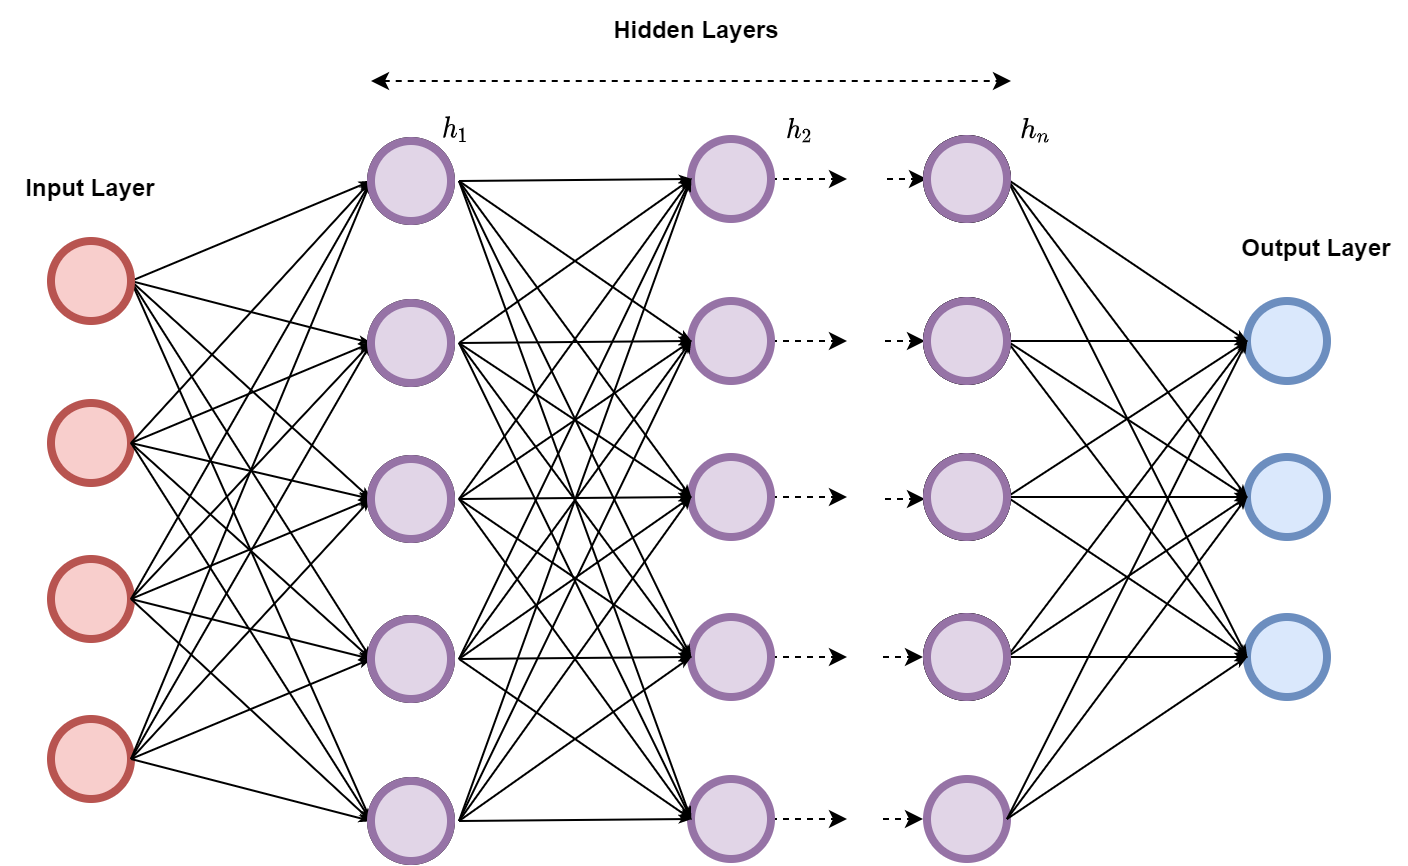
\includegraphics[scale=0.2]{theory/ann.png}
\caption{An illustration of neural connections in an ANN}
\label{fig:ann}
\end{figure}

The input layer consists of the input features/data vector. There are connections between every neuron in the hidden layer and the input layer. Every connection carries an associated weight that transforms the input to the output of every neuron as below:
\begin{equation}
\begin{split}
    a^1_{j}&=\sigma(\sum_{i=1}^{n_f}(X_iW^1_{i,j}) + b^1_j)\\
    \sigma(x)&=\frac{1}{1+\exp(-x)}\\
\end{split}
\end{equation}
Here $a^1_j$ is the output at the $j^{th}$ neuron of the first hidden layer and $n_f$ is the number of input features. $W^1_{i,j}$ refers to the weights between the input and the first hidden layer, whereas $b^1_j$ refers to the bias of the $j^{th}$ neuron in the hidden layer. A non-linear activation function is used to transform a linear transformation of the the input $X_i$ to the output $a^1_{j}$. The non-linear activation used above is a sigmoid activation. Many other activation functions such as tanh, ReLU can also be used.  The purpose of these activations is to obtain a non-linear transformation of the input $X_i$. An ANN further consists of multiple hidden layers that perform similar transformations to $a^1_{j}$. The final layer of an ANN is called as the output layer as it takes the output  obtained from the last hidden layer and transforms it to a vector, which has the same dimensions as the target feature. Therefore, there are connections between each neuron in the last hidden layer to every neuron in the output layer as below:
\begin{equation}
\begin{split}
    a^l_j&=\sigma(\sum_{i=1}^{n_l}(a^{l-1}_iW^l_{i,j}) + b^l_j)\\
\end{split}
\end{equation}
Here $n_{l-1}$ refers to the size of the last hidden layer $l-1$ and the output at the $j^{th}$ neuron is calculated as the dot product of the hidden layer output with the output neuron weights added to the bias of the output neuron. An activation function may/ may not be applied here, depending on the target feature. If the target feature is categorical, it may be useful to use a sigmoid function activation that squishes the values between 0 and 1. This entire transformation of input through multiple hidden layers and activations to the final output is termed as a forward pass. 

Most of the ingenuity in an Artificial Neural network lies in tuning the weights and biases of these networks, given the target data. Having computed the "predicted" outputs from the forward pass, it becomes paramount to construct some error metric to gauge the difference between predicted and actual target vectors. For the problem of regression, a simple mean squared error metric can be utilized. The problem can now be termed as minimizing this loss function/error metric, by fine-tuning the weights of the network. This loss function represented by $F(x)$ is multi-variate, as it is dependent on many weights and biases. The loss function reduces the fastest in the direction of its negative gradient. Using this observation, the weights can be updated as below
\begin{equation}
    \begin{split}
        W_{n+1}=W_n-\alpha\nabla F(W_n)
    \end{split}
\end{equation}
$\alpha$ signifies the learning rate which represents the size of the steps taken towards reaching the minima. In the above equation, it will thus be necessary to compute the gradients of the objective function with respect to each of the weights and biases. For this, gradients of loss are computed with respect to the activations of the final layer. Using the chain rule of differentiation, the gradients of loss with respect to the previous hidden layer's weights and biases can be computed. 

\begin{equation}
    \frac{\partial F}{\partial W^l_{j,k}}=\frac{\partial F}{\partial a^{l}_{j}}\frac{\partial a^{l}_{j}}{\partial W^{l}_{j,k}}\\
\end{equation}

The chain rule can be applied multiple times to compute gradients backwards for all weights and biases. This part of tuning the weights is referred to as backpropagation and is responsible for training the network. 

The idea for training the network is to compute the loss function for the entire data (such as MSE for the entire data) and then use backpropagation to tune the weights and repeat the process until convergence. However, this becomes computationally slow and also requires loading the entire dataset into the memory. On the other hand loss and gradients can only be calculated for every data point in our dataset and gradient updates can be made for every forward pass. This is called as stochastic gradient descent\cite{Robbins&Monro:1951}, but this gives noisy updates to the parameters. In practise, the solution is to combine these two ideas to feed-forward min-batches of data through the network. For every mini-batch, loss and gradients are computed and weights are updated. A complete pass through the entire dataset is called an epoch. The network is trained through multiple epochs until the error estimate/loss function starts converging. 

\subsubsection{Recurrent Neural Networks}
The working of a recurrent neural network (RNN) shares similarities to the working of an Artificial Neural Network. Both ANNs and RNNs contain layers and activation functions with many parameters that are tuned to approximate the target variable $Y$ as a function of input features $X$. However, the standard ANN cannot be used to model temporal dependencies in the data. RNNs on the other hand have proven to be a modern standard in dealing with time series data. The intuition behind how RNN deals with temporal data can be understood by borrowing some concepts studied in the Kalman Filter section. In the Kalman Filter, there is a hidden state that affects the measured output. At the same time, the hidden state itself is temporal in nature as the next hidden state is dependent on the previous hidden states. As a result of this cross-dependence, the output states themselves are temporally related to each other. The Elman network \cite{miikkulainen_simple_2010} introduced in 1990 which is one of the most widely used RNN variant uses this concept of a hidden state to good use. 
\begin{equation}
\begin{split}
    h_t&=\sigma_h(W_hx_t+U_{h}h_{t-1}+b_h)\\
    y_t&=\sigma_y(W_yh_t+b_y)
\end{split}
\end{equation}
where $W_h$, $U_h$, $W_y$, $b_h$,$b_y$ represent parameter weight,bias vectors and $\sigma_h$,$\sigma_y$ represent activation functions. 

\begin{figure}[H]
\centering
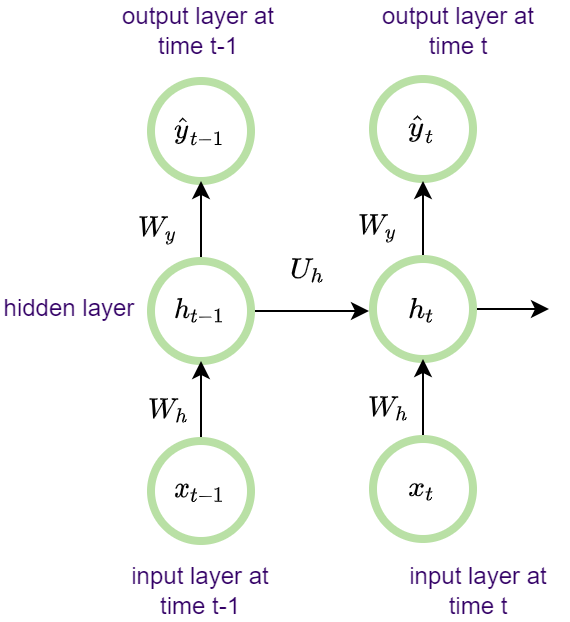
\includegraphics[scale=0.4]{theory/rnn.png}
\caption{A time unfolded representation of the Elman Network}
\label{fig:rnn}
\end{figure}
As can be seen there is a hidden layer at time $t$ which is dependent on the input at time $t$ and the hidden layer from the previous time $t-1$ through activation functions and respective weights. The previous hidden layer acts as some sort of memory/ past context which when coupled in a specific way with the present input, gives the present context. This present context $h_t$ influences the output $y_t$ through more such weights and activation functions. $W_h$ controls the amount of information that should be passed from the input to the hidden state. Similarly, $U_h$ controls the information flow between past and present hidden state. Lastly $W_y$ dictates the information flow between the hidden state and the output vector. The same parameter vectors are used for each time step $t$. Thus, through these hidden states, the network develops some sort of a memory through which time is represented via its effect in intermediate computations. The network's parameters are trained using the same backpropagation principles present in an ANN. 

RNNs have been used with high degrees of success on a variety of tasks. However, the novel idea used in an RNN to unroll the network across multiple time steps also proves to be its downfall. As the number of time-steps increases, the network is unrolled over many layers. Let us say that the output at the last layer was dependent on the first one. When the network tries to learn this dependency and the gradients at the last layer are small, the gradients vanish as we move backwards through the many layers present in the network.  This is referred to as the vanishing gradient problem \cite{pascanu_difficulty_2013}. As a result, earlier layers don't learn and the signal is lost. On the other hand if the gradients begin large at the last layer, gradients will get larger as they are backpropagated through to the input. Therefore, the weights near the input layer will be large and as a result will forward propagate larger signals, making the error estimates very large. This is known as the exploding gradient problem. The mathematics of gradient vanishing and explosion are present in \cite{pascanu_difficulty_2013}. In conclusion, Elman Networks were successful in solving relatively simple problems and as sequences scaled up in size and complexity, these networks frequently struggled. 

\subsubsection{Long Short Term Memory}
Long Short Term Memory (LSTM) networks \cite{HochSchm97}, introduced in 1997 was designed to combat many of the problems that RNNs were facing. LSTMs are special kinds of RNN architecture that operates in the same loop-like way of an RNN. However the architecture of an LSTM cell is markedly different as it has a gated circuit that controls information flow from previous time step to current time step.
\begin{figure}[H]
\centering
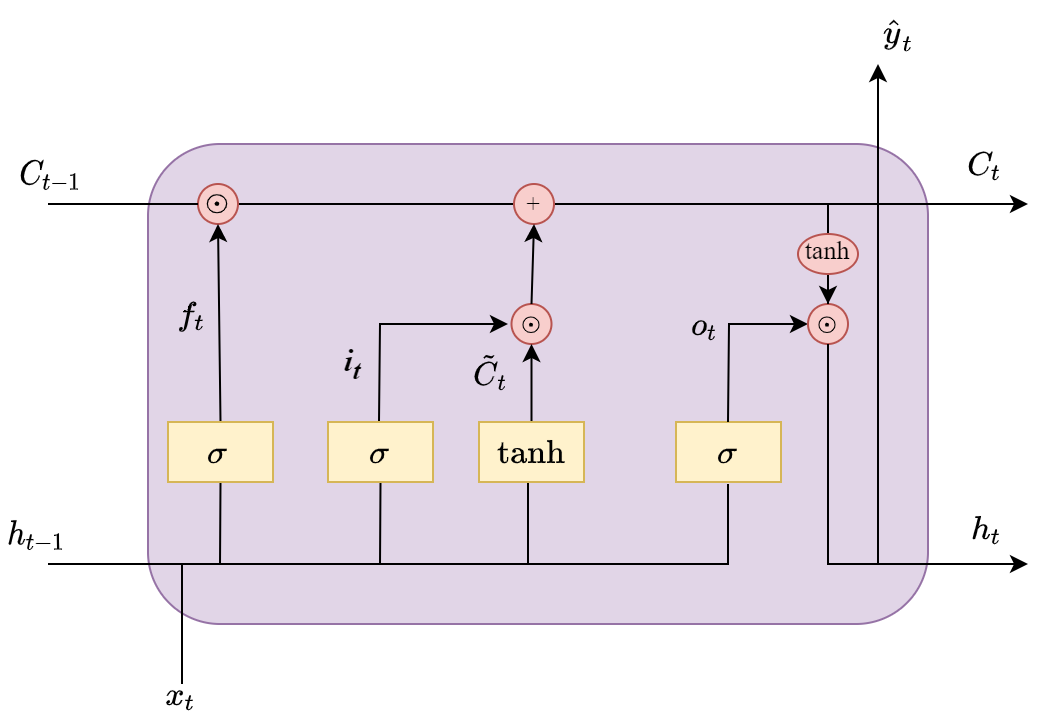
\includegraphics[scale=0.4]{theory/lstm-cell.png}
\caption{LSTM gated architecture}
\label{fig:lstm}
\end{figure}


In the figure above, the rectangular boxes are fully connected layers with trainable parameters. The circular boxes refer to element-wise operations between different vectors. $h, x $ and $C$ refer to the hidden state vector, input feature vector and the cell state vector respectively. The LSTM can be thought of as making three separate decisions at each time step: forget/keep information, update information and output information using the memory. To understand these three decisions, a forward pass in this LSTM is elaborated upon.
\begin{itemize}
    \item Firstly, the feature vector  from the current time step ($x_t$) and the previous hidden state vector ($h_{t-1}$) are concatenated. For convenience, this concatenated state is referred to as the concatenated input vector from here on.  This concatenated input vector is passed through a feed forward layer with a sigmoid activation. The output from this activation is later element wise multiplied with the previous cell state. The purpose of this stage (also called the input gate) is to forget irrelevant information from the previous state. 
    \begin{equation}
    \begin{split}
        f_t&=\sigma(W_f\cdot[h_{t-1},x_t]+b_f)
    \end{split}
    \end{equation}
    \item Secondly, the concatenated input vector is passed through two feedforward layers: one with sigmoid activation and another with tanh activation. The output from the tanh function decides the update that should be passed into memory for each value and is termed as candidate memory. The output from the sigmoid activation, also referred to as the input gate decides which values needs to be updated. The element wise multiplication of the candidate memory and the input gate combines update information and updates only specific values in this vector. The present cell state is the sum of what we decided to keep from the previous cell state and the updates from the new concatenated input vector. 
    \begin{equation}
        \begin{split}
            i_t&=\sigma(W_i\cdot[h_{t-1},x_t]+b_i)\\
            \tilde{C_t}&=\tanh(W_C\cdot[h_{t-1},x_t]+b_C)\\
            C_t&=f_t*C_{t-1}+i_t*\tilde{C_t}
        \end{split}
    \end{equation}
    \item Lastly, the concatenated input vector is passed through another feedforward layer with a sigmoid activation, also referred to as the output gate. The tanh function is applied on the cell state and the vector from the output gate is element wise multiplied to obtain the new hidden state. This essentially regulates what information from the cell state needs to be passed on to the hidden state.
    \begin{equation}
        \begin{split}
            o_t&=\sigma(W_o[h_{t-1},x_t]+b_o)\\
            h_t&=o_t*tanh(C_t)
        \end{split}
    \end{equation}
    
\end{itemize}

It can be shown that in these kinds of gated units, the gradients don't vanish exponentially fast because of the cell state and that's why it becomes pertinent to use LSTMs in long-trajectory time-series methods. 

\subsubsection{Self Attention and Transformer Encoders}\label{ssec:transformers_theory}
Self attention was a concept first discussed in \cite{vaswani_attention_2017}, which aimed at computing similarity scores between words in a sentence. For example in the sentence "John went to the store because he wanted milk", the word "he" needs to be associated with "John". Self attention is the mechanism through which the model understands these kind of inter-sentence dependencies. In our case, we have multiple road users traversing and each of their behaviors is influenced by some other road user's behavior. Therefore it becomes important to try and bake these inter road user dependencies in the model.  We propose to use the self attention mechanism in our problem through a transformer encoder architecture. The transformer encoder architecture was introduced in the same paper, where the transformer was used to process an entire sentence as a whole in a non-recurrent fashion. The recurrent nature of LSTMs or RNNs made their performance dependent on whether the hidden state was preserving information from previous time steps. By processing entire sequences as one, the Transformer architecture had no risk of losing past information. Transformers have revolutionized the field of natural language processing and computer vision, because of their capability to adapt to different tasks. Through this section, this architecture and its constituent building block of self attention will be discussed in detail. 


\begin{figure}[H]
\centering
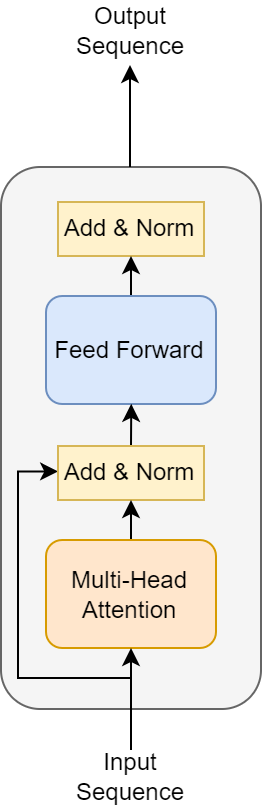
\includegraphics[scale=0.4]{theory/transformer.png}
\caption{Transformer Architecture}
\label{fig:transformer}
\end{figure}

The transformer encoder architecture consists of a self attention layer followed by a feed forward layer. Let us say that the input to the transformer architecture is a feature vector, where a feature vector somehow represents the individual behavioural state of one road user. At a particular point of time, we may have multiple road users and thus a collection of feature vectors collected into a matrix. Let us assume that there are $p$ feature vectors and $d$ is the dimension of each feature vector also called as the embedding dimension. 
\begin{equation}
    \begin{split}
        Q&=XW_Q\\
        K&=XW_K\\
        V&=XW_V\\
    \end{split}
\end{equation}
The feature matrix ($X$) we have is firstly multiplied with three trainable parameter matrices $W_Q$, $W_K$ and $W_V$. Each of these matrices have a dimension of $d \times w$. Therefore for each feature vector we obtain a query vector, a key vector and a value vector. As a matrix, we obtain the query ($Q$), key ($K$) and value matrices($V$) of dimension $p \times w$. 

Next, the query matrix is multiplied with the transpose of the key matrix. To understand the intuition behind this, let us say that $p=2$ or that there are two feature vectors. Therefore the resulting $QK^T$ will be a $2 \times 2$ matrix. 
\begin{figure}[H]
\centering
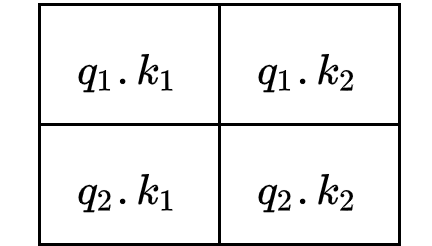
\includegraphics[scale=0.4]{theory/example.png}
\caption{An illustration of $QK^T$ for a $2 \times 2$ matrix}
\label{fig:transformer-example}
\end{figure}


The first cell (1,1) of this matrix is the dot product between the query vector of the first feature  and the key vector of the first feature. This can be thought of as the score that first feature vector gives itself. It becomes more interesting when we look at the second (1,2) and third cell (2,1).
The second cell is the dot product between the query vector of the first feature and the key vector of the second feature. This can be thought of as the score/importance that the first feature gives to the second feature. Similarly the third cell is the score/importance that the second feature gives the first feature and the fourth cell is score/importance the second feature gives itself. Therefore, the resulting matrix represents the importance/attention that every feature vector gives every other feature vector. This entire matrix is divided by the square root of the dimension of the key vectors, that serves a more practical purpose of having stable gradients. Then the softmax function is applied over the resulting matrix to normalize the scores into some kind of a probabilistic distribution. The row sum of the resulting matrix is 1 and each cell of a row represents how important that particular cell is for the row. 

Now the resulting normalized score matrix obtained is multiplied with the value matrix. Essentially every row of the resulting matrix is the weighted sums of different feature's value vectors, weighted by the normalized score of a feature. The $n^{th}$ row will consist of the sum of the weighted value vectors of each feature, weighted by their importance relative to the $n^{th}$ feature. 

\begin{equation}
    \begin{split}
        Z=softmax(\frac{QK^T}{\sqrt{d_k}})V
    \end{split}
\end{equation}

There can also be multiple-attention heads where there are multiple $W_Q$, $W_K$ and $W_V$ matrices for each attention head. As a result we would obtain $Z_1, Z_2 ... Z_{natt}$ as the output of these attention heads. These outputs are concatenated and multiplied with another trainable parameter $W_O$ to obtain $Z_{net}$

\begin{equation}
    \begin{split}
        Z_{net}=W_o(concat(Z_1,Z_2...Z_{natt}))
    \end{split}
\end{equation}

Each feature vector in the $Z_{net}$ matrix is then passed through two feed-forward layers, with the first feed-forward layer having a ReLu activation to obtain $Z_{out}$. The input and the output of both the multiple-attention head layer and the feed-forward layer are added and layer normalization is applied. These connections between the input and the output is termed as a residual connection and is implemented for the practical purpose of limiting the vanishing gradient problem. At the end of the transformer encoder, an output feature vector is produced for each feature vector input. The $n^{th}$ output feature vector incorporates information from all the input features with respect to the $n^{th}$ input feature vector. The details regarding how these neural network architectures are implemented for the specific problem in our thesis is elaborated in the section \ref{ssec:tlstm}\ref{ssec:vanilla_lstm} 

\section{Data}
Through this section, we present details regarding the features, quantity and quality of data. Further, through data exploration and visualization, key facets and characteristics of the data is presented. Lastly, important pre-processing steps that suitably mould the data for later algorithms are enumerated. 

The data has been supplied by Viscando, whose technology tracks all road users to understand movement patterns, traffic flow and human behaviour. Installed on static road infrastructure like light posts or building walls, Viscando’s sensor OTUS3D detects, classifies, and tracks all road users using 3D vision and AI. Images simultaneously captured by two spatially separated cameras are converted into a dense 3D point cloud. Point clustering is then applied to the point cloud to detect single road users and to estimate their sizes and 3D shapes. Then, the objects are classified using shape- and appearance-based AI methods. Finally, object tracking using Kalman filter is applied to compute trajectories of different objects, with time-resolved position, speed, acceleration and heading.In case the measurement system consists of several sensors, the detections from individual sensors are merged before tracking. Two such vision sensors were placed on the buildings of the Link\"{o}ping University campus. The data collected over a week contains trajectories of pedestrians, cyclists and the autonomous shuttles. 



\begin{figure}[H]
\centering
\begin{subfigure}{.5\textwidth}
  \centering
  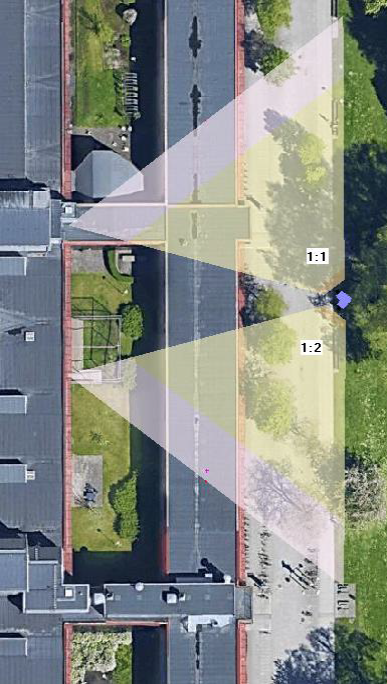
\includegraphics[width=.6\linewidth]{data/Data_1.png}
  \label{fig:sensor}
\end{subfigure}%
\begin{subfigure}{.5\textwidth}
  \centering
  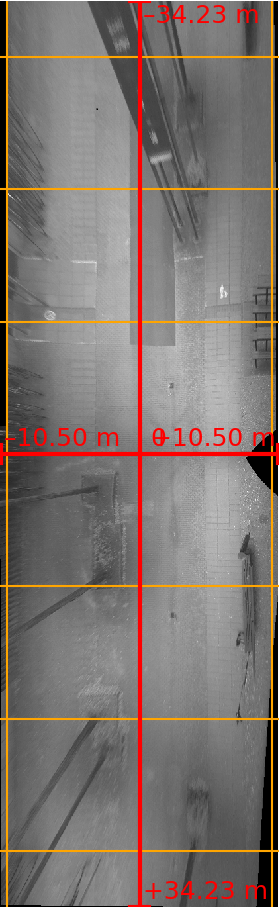
\includegraphics[width=.325\linewidth]{data/ground.png}
  \label{fig:top_view}
\end{subfigure}
\caption{Top view of sensor placement and sensors' field of view}
\label{fig:sensor_view}
\end{figure}


\begin{figure}[H]
\centering
\begin{subfigure}{.3\textwidth}
  \centering
  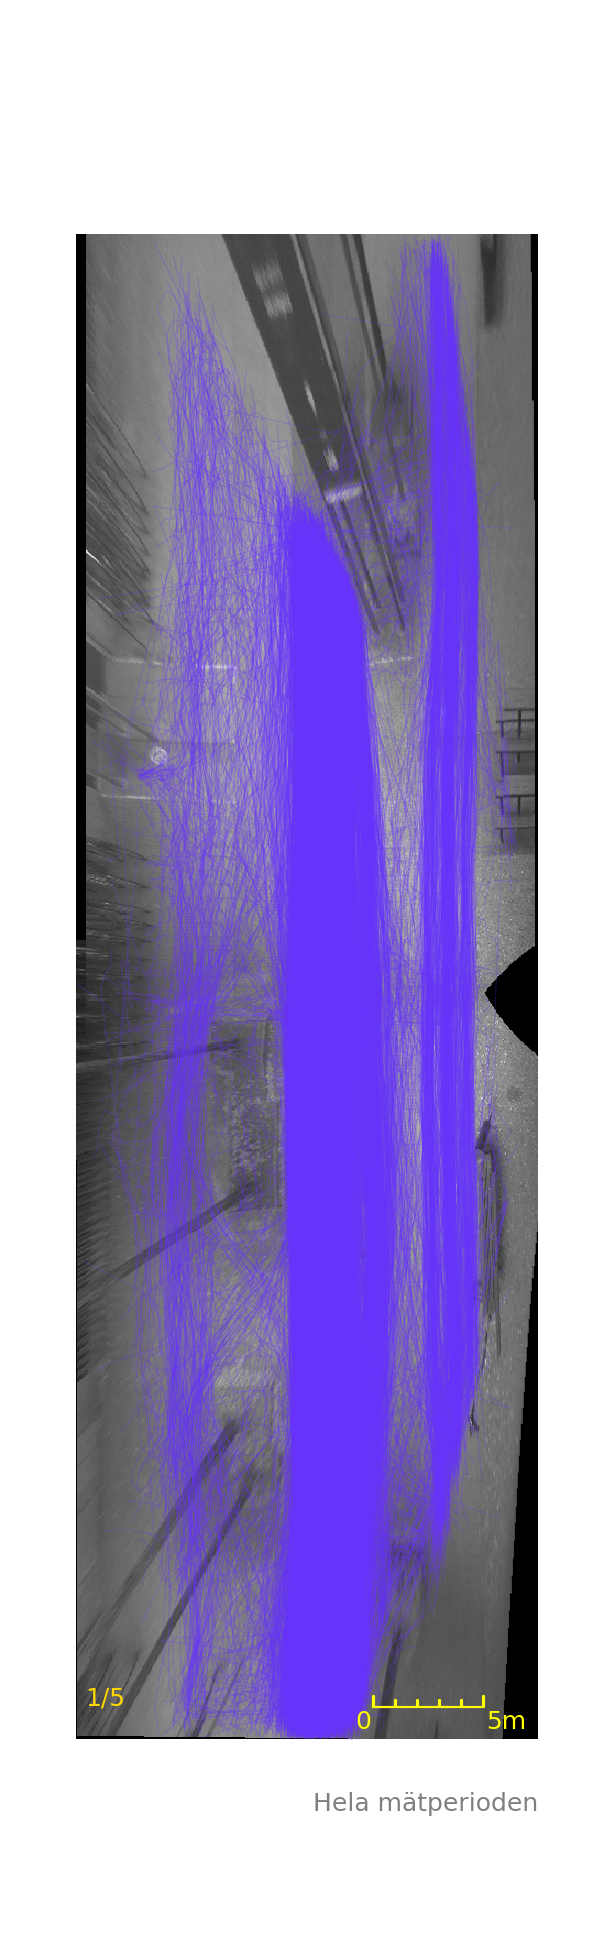
\includegraphics[width=\linewidth]{data/Data_2.png}
  \caption{Cyclists}
  \label{fig:cyc_tra}
\end{subfigure}%
\begin{subfigure}{.3\textwidth}
  \centering
  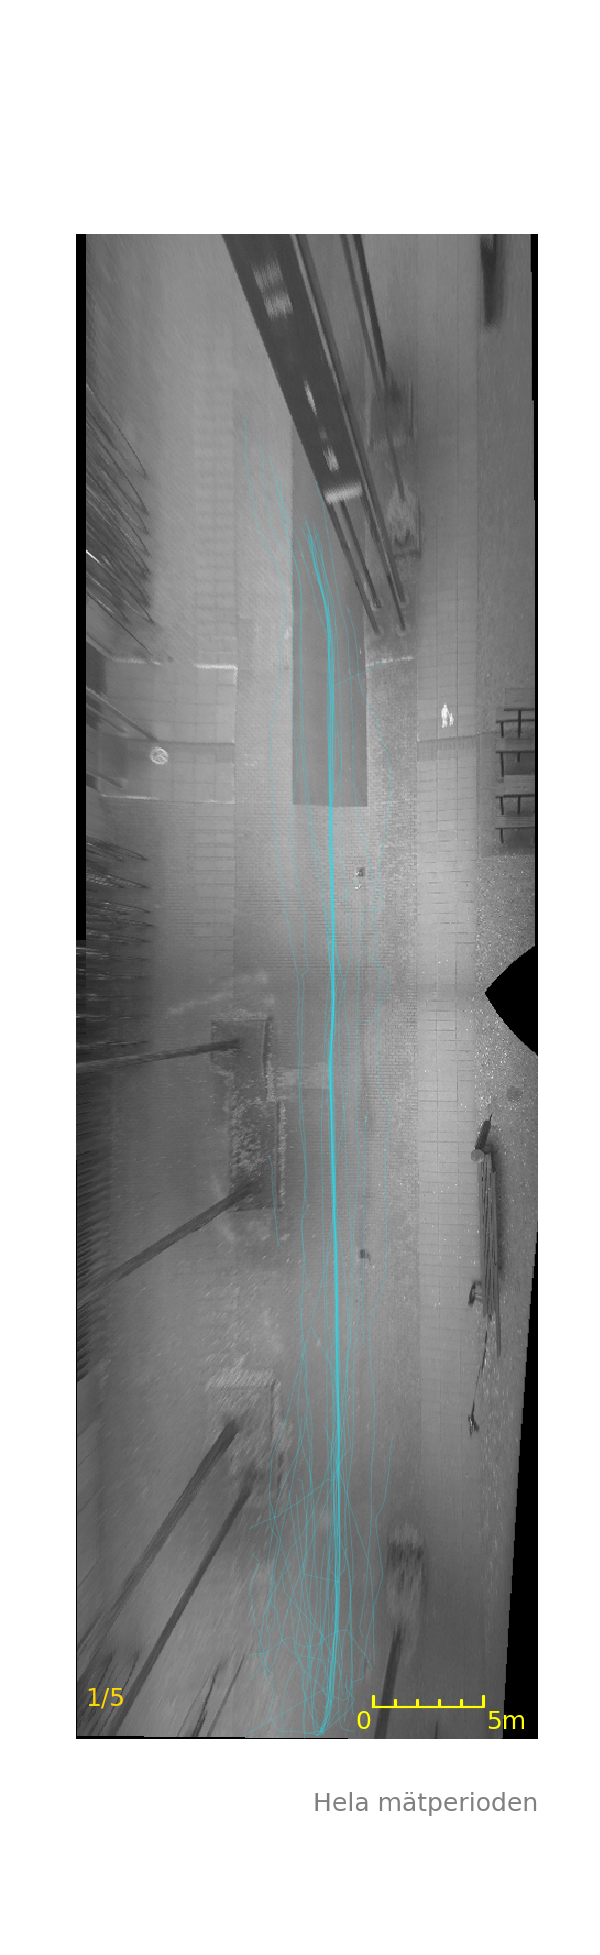
\includegraphics[width=\linewidth]{data/Data_3.png}
  \caption{Shuttles}
  \label{fig:shu_tra}
\end{subfigure}
\begin{subfigure}{.3\textwidth}
  \centering
  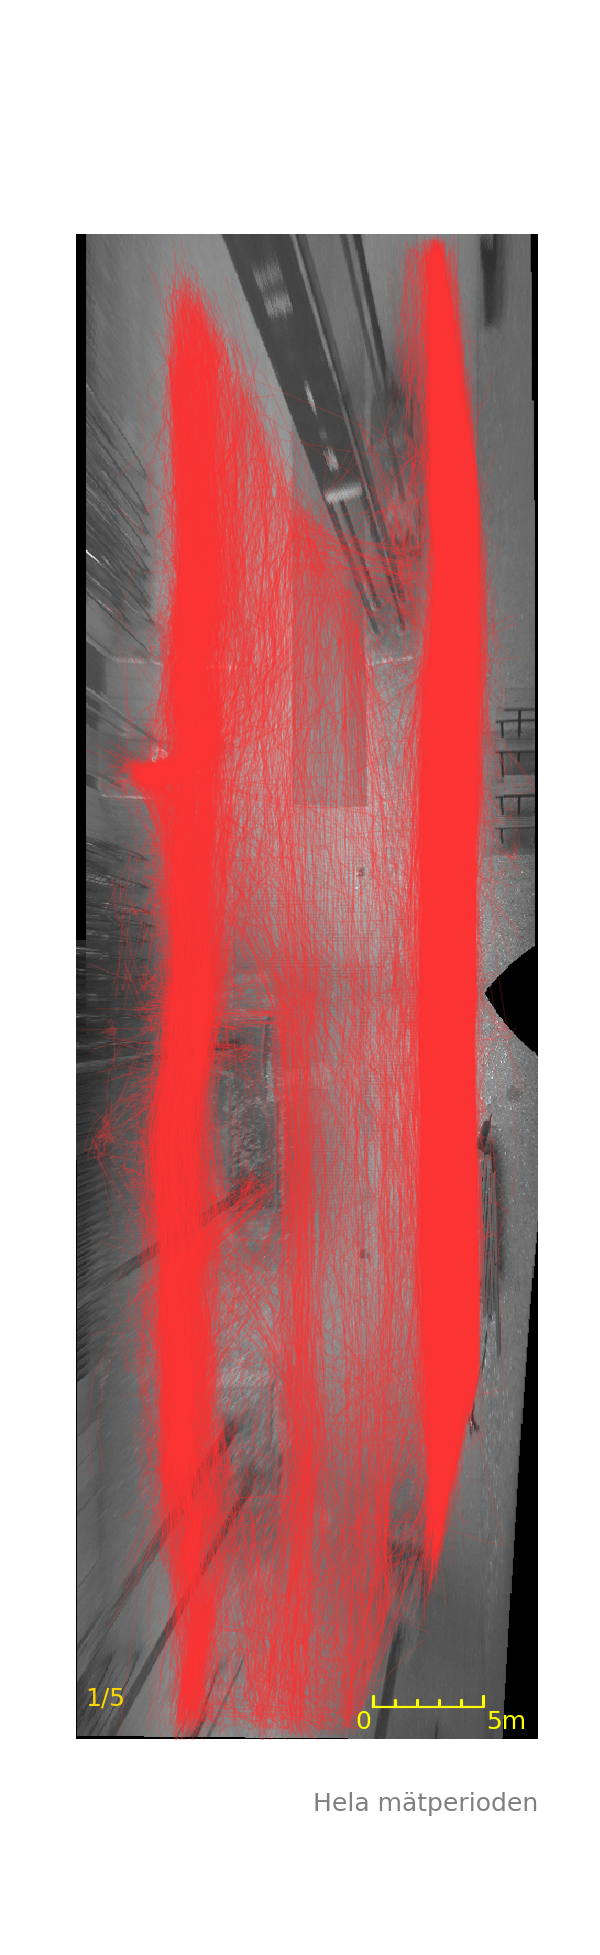
\includegraphics[width=\linewidth]{data/Data_4.png}
  \caption{Pedestrians}
  \label{fig:ped_shu}
\end{subfigure}
\caption{Line plots for trajectories of road users}
\label{fig:trajectories}
\end{figure}

As can be seen from Fig. \ref{fig:sensor_view}, the field of vision of the sensor covers an area of $70 \times 21$ metre squared. 

\begin{figure}[H]
\centering
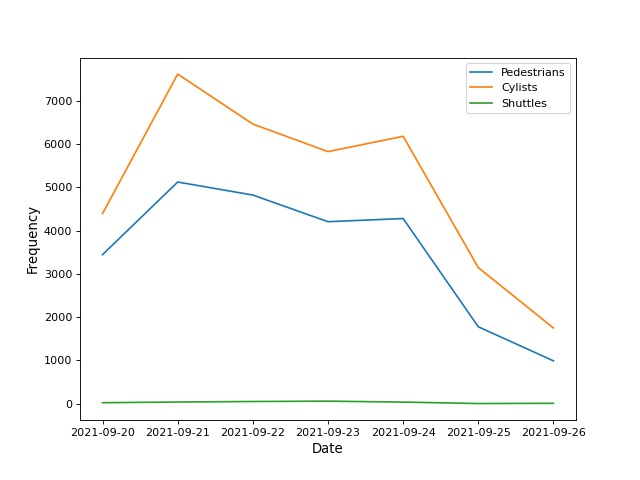
\includegraphics[scale=0.3]{data/Data_6.jpg}
\caption{Top view of sensor placement and sensors' field of view}
\end{figure}



The feature names along with their definition and type are tabulated below:
\begin{table}[H]
\begin{center}
\begin{tabular}{ cccc } 
\hline
Feature Name & Definition & Variable type\\
\hline
ID & Unique ID assigned to each road user & Continuous\\ 
Timestamp & Time at which road user was tracked & Time\\ 
x & Tracked X-Coordinate of a road user & Continuous\\
y & Tracked Y-Coordinate of a road user & Continuous \\
Speed & Tracked speed of a road user&Continuous \\
Type & Indicator for cyclist, pedestrian and shuttle & Categorical\\
\hline
\end{tabular}
\caption{\label{tab:features}Definition and type of variables in the dataset}
\end{center}
\end{table}


\begin{table}[H]
\begin{center}
\begin{tabular}{ cccc } 
\hline
Type & No. of trajectories & Avg speed (km/h) & Avg Trajectory Length (s)\\
\hline
Pedestrians & 24639 & 4.6 &30\\ 
Cyclists & 35373 & 14.0 &13\\ 
Shuttles & 208 & 6.6 &21\\
\hline
\end{tabular}
\caption{\label{tab:road-user}Characteristics of each road user in the dataset}
\end{center}
\end{table}




\subsection{Data Manipulation}
Through the analysis of sampling times, there was an interesting observation made. Sampling time is defined as the time difference between any two consecutive observations for the same road user. It can also be thought of as the inverse of sensor frequency, where the sensor frequency is defined as number of frames captured per second. The table below shows the distribution of sampling time in the data.



\begin{table}[H]
\parbox{.45\linewidth}{
\centering
\begin{tabular}{@{}cccc@{}}
\toprule
Sampling Times (in seconds) & Frequency\\ \midrule
Between 0.05 and 0.2 & 3540\\ 
0.24 & 822904 \\  
Between 0.3 and 1.5 & 8524 \\  
Greater than 1.5 & 4472 \\
\bottomrule
\end{tabular}
\caption{Distribution of sampling times}
\label{table:sampling_time}
}
\hfill
\parbox{.45\linewidth}{
\centering
\begin{tabular}{@{}cccc@{}}
\toprule
Times & User 1 & User 2 & User 3 \\ \midrule
09:10:40:00  & $[x_1,y_1]$ & $[x_2,y_2]$ & $[x_3,y_3]$ \\
09:10:40:20 & $[x_1',y_1']$ & $[x_2',y_2']$ & $[x_3',y_3']$\\
09:10:40:40 & $[x_1'',y_1'']$ & $[x_2'',y_2'']$ & $[x_3'',y_3'']$\\
09:10:41:00 & $[x_1''',y_1''']$ & $[x_2''',y_2''']$ & $[x_3''',y_3''']$\\
\bottomrule
\end{tabular}
\caption{Aligned road users' data}
\label{table:common_axis_data}
}
\end{table}


It is seen that the sampling time is not constant throughout the data. Most of the data has a sampling time of 0.24 seconds. However, there are cases where the sampling time is higher/lower. It is important to maintain a constant sampling time, because then we can have a common time axis for all road users. Then, one can align different road user's data as Table \ref{table:common_axis_data}, and at any particular time, the positions of all road users in the frame are known. In order to make the sampling time uniform, positions and speeds of road users need to be calculated for a common time scale. It was decided to choose a time scale of 0.2 seconds because of its proximity to the most frequent sampling time (0.24 seconds) and for convenience. Let us say a road user's position was known at 0.24, 0.48,0.72, 0.96 seconds the road user's position at 0.2, 0.4, 0.6, 0.8 and 1 second needed to estimated. Simple cubic interpolation was used to interpolate positions and speeds to the nearest $0.2^{th}$ second. Now the data had a uniform sampling time of 0.2 seconds. By taking the $5^{th}$ observation of every road user, dataset with a sampling time of 1 second was also  created.  Thus, there were two final datasets each with sampling times of 0.2 second and 1 second respectively. 

\subsection{Data processing for recurrent neural networks}

Every road user maps out a trajectory which keeps evolving as the road user moves through the frame. In order to predict where the road user will be in the future, his/her past trajectory is of utmost importance. Therefore, it is desired that the network predicts the coordinates at time step $t+s$ given the input trajectory until time $t$. For the network to be able to do its best job predicting, data needs to be packaged in an $[input^{1}_t,target^{1}_t]$ fashion where input represents what the network needs to know about road user 1 in order to predict the target. The input trajectory of a road user 1 at time $t$ consist of feature representations from each time step $1,2,...t$  of his/her trajectory . In turn each of these feature representations at time $k$ are the road user's position ($x^1_k,y^1_k$) and two dummy variables ($ped,shu$) signifying whether the road user is a pedestrian or cyclist. Notice that these two dummy variables will be the same for each time step $t=1,2...n$. The target feature is the position of road user s steps later, or in other words, $x^{1}_{t+s},y^{1}_{t+s}$  needs to be predicted. The data structure also called as the \textit{Individual Trajectories} data structure will consist of two columns $[input,target]$ and the equations below help in understanding how each row of $[input,target]$ will look like Eq. \ref{eq:lstm_data} . The Kalman Filter EM Algorithm and the Vanilla LSTM network introduced later in section \ref{ssec:CV_model}, \ref{ssec:vanilla_lstm} will be trained on this data structure after applying some exclusions that is mentioned later in \ref{ssec:exclusions}. 
\begin{equation}\label{eq:lstm_data}
    \begin{split}
        input^{1}_t&=[[x^{1}_1,y^{1}_1,ped,shu],[x^{1}_2,y^{1}_2,ped,shu],...[x^{1}_t,y^{1}_t,ped,shu]]\\
        target^{1}_t&=[x^{1}_{t+s},y^{1}_{t+s}]
    \end{split}
\end{equation}
If the data is structured in a different way, there is more information that can be leveraged. In the above representation, the input features at time $t$ consist of a road user's past trajectory and the target feature consists of the road user's future trajectory. However, at  time $t$ there may be $m$ multiple road users in the scene, influencing each other's behaviour. At time $t$ it would certainly be more interesting to tell the network that there are other road users in different coordinates at the same time. Thus, the input feature needs to be packaged such that all the current road users' trajectories are present. Consequently the target feature should consist of all the road users' future coordinates. Therefore the representation of the entire scene (and not just one road user) at time $t$ $[input_t,target_t]$ will look as in Eq. \ref{eq:transformers_data}. The data structure called as the \textit{Frames} data structure will consists of multiple rows of such frames and the Attention based LSTM network introduced later in \ref{ssec:tlstm} will be trained on this kind of a data structure. 
\begin{equation}\label{eq:transformers_data}
    \begin{split}
        input_t&=[input^{1}_t,input^{2}_t...input^{m}_t]\\
        target_t&=[target^{1}_t,target^{2}_t,...target^{m}_t]
    \end{split}
\end{equation}
where $input^{k}_t$ and $target^{k}_t$ is obtained from the equation \ref{eq:lstm_data}

\subsubsection{Data Exclusions}\label{ssec:exclusions}
There are some exclusions applied to the data and the reason for applying these exclusions are elaborated in this section. 

When analyzing the distributions of speed, there were some observations which had a very high speed ($>$50 kmph). On further analysis, it was seen that this happened mostly at the start frame when the road user was captured.  It is important to know that in the data given to us, the first three frames of the tracked road user is discarded as they will contain noisy tracked estimates of positions and speeds. Speeds are derived from previous positions and sometimes it may be the case that speed estimate in the fourth frame is also noisy, because uncertainty in measuring speed is higher than uncertainty in measuring position. Therefore,  for safe measure these road users ($<0.5\%$) are discarded in our analysis.

It is also mandated that the trajectory of a road user consists of at least two seconds (which is two timesteps steps in a 1 second sampled data and 10 timesteps in a 0.2 second sampled data) for future predictions. This is done so that there is enough input to the network, before a network starts predicting. This serves the purpose of eliminating noise from too few observations to make a prediction. This exclusion is applied to all these datasets. 

There are some interesting cases when making the \textit{Frames} data structure. There may be three road users at the time of observation, but $s$ time steps later, one of them (or all) may have left the frame. In this case for the missing road user who left the frame, the target features are populated as NaNs (not a number/missing value). As mentioned later in Section \ref{ssec:tlstm}, the network does not calculate loss over these cases. There may be also be cases where a new road user entering the scene has just one second of data, whereas all other road users have history that extends multiple seconds into the past. Thus, one row of the \textit{Frames} data structure has some road users with a good past and some road users without the minimum two seconds.  One option here would be to remove this new road user from the observation (input) and prediction (target). However, that road user, even with one observation, may be influencing the scene. Therefore his/her data removal may violate the natural social structure present in the scene. In order to avoid this problem , that entire timestamp's scene is removed from the data $[input_t,target_t]$. In the next timestamp, this new road user will have two prior timesteps of features and if no other road users freshly enter the scene, this scene is included for training. This step doesn't exclude entire road users' trajectories, but predictions are not performed on some time steps in these road users' trajectories. 

Another interesting case that is observed in the \textit{Frames} data structure is that two pedestrians/ two cyclists are very close to each other throughout their trajectory. Sometimes the distance between the two road users is 0 throughout the trajectory. This means that one of the road users was detected as two road users. These kinds of observations were removed from the dataset. Also, two road users can be quite close to each other when they are walking. For example, if acquaintances are walking together, they do not maintain a lot of distance between them. A heuristic cutoff of 20 cm is used as the minimum distance between any pair of road users throughout their trajectory. This means that if two road users maintain a distance of less than 20 cm throughout their trajectory, only one road user is considered as we assume that two road users were detected as one. Through this cutoff, $<1\%$ of road users were removed. 

After all the cleaning, roughly 25\% of road users were removed, of which most of them had a very short trajectory length ($<$ 2 seconds).  The \textit{Individual Trajectories} data structure can be used for the Kalman Filter training and for the Vanilla LSTM network. The \textit{Frame} data structure can be used for the attention based LSTM network's training as this network tries to model the social behavior. To make matters more convenient, the trajectories present in the \textit{Frames} data structure is used to train the Kalman Filter network, LSTM network and the Attention based LSTM network. This is because it would be interesting to see how these methods compare when trained on the same data.

\section{Methodology}
In this section, the rationale behind choosing the methods mentioned in the theory is elaborated. Further implementing this theoretical method on the specific data is presented in more detail. 

\subsection{CV Model and the Kalman Filter}\label{ssec:CV_model}

The data as we have studied in the previous section consists of pedestrians, cyclists and shuttles. The trajectories of all these road users are present from the moment they were detected by the sensors to the moment their detection was stopped. These trajectories themselves are temporal in nature as the position in the future is correlated with the position in the past. Multiple trajectories thus can be treated as multiple time series/autoregressive sequences. A solution often used when dealing with time-series specific problems is the Kalman filter. The Kalman filter as mentioned in \ref{ssec:kf_theory} constructs dependencies between a latent variable and an observed variable. 

\begin{equation}\label{eq:m1}
\begin{split}
    X_{t}=AX_{t-1} + \eta_t\\
    Z_{t}=CX_{t}+\epsilon_t\\
\end{split}
\end{equation}
where $\eta_t$ and $\epsilon_t$ are distributed as $N(0,Q)$ and $N(0,R)$ respectively. 

From the above equation, we see that the latent variable has temporal dependencies and the observed variable is a function of the latent variable. If the model parameters and the hidden states in Eq. \ref{eq:m1} are known, one can calculate the future hidden states and future observed states. The advantage of a Kalman filter is that one can make n-step predictions not only about the means of the observed states, but also the uncertainty around the observed states. This makes the Kalman Filter useful in calculating predictions ahead of time. In the case of our problem, the latent variable is assumed to be the actual positions and speeds of a road user. The observed variable is the measured position that is obtained from the data. This setting along with specific parameters for $A$ and $C$ is used in the Constant Velocity model. 

$$X_t=\begin{pmatrix}x_t 
\\ \dot{x_t} 
\\ y_t 
\\ \dot{y_t} 
\end{pmatrix}, 
A=\begin{pmatrix}1 & \Delta t & 0 & 0 
\\ 0 & 1 & 0 & 0 
\\ 0 & 0 & 1 &\Delta t
\\ 0 & 0 & 0 & 1 
\end{pmatrix}
Z=\begin{pmatrix}
Z_{x_{t}}\\
Z_{y_{t}}\\
\end{pmatrix}, 
C=\begin{pmatrix} 1 & 0 & 0 & 0\\
0 & 0 & 1 & 0\\
\end{pmatrix}
$$

The constant velocity model has been extensively used in the object tracking literature. The tracking problem deals with obtaining noise free estimates of positions given noisy sensor measurements of an object's position. The constant velocity model is considered as a robust method for tracking (insert reference) and can also be extended to prediction. This has already been done before (insert reference) and this model is also considered as a solid, robust baseline for intent prediction. For all these reasons, it was decided to go ahead with a CV model albeit with a slight change in implementation. 

The values of $Q$, $R$ are usually empirically chosen in CV models. However, in this paper we aimed to estimate $Q$, $R$ through data driven approaches. This was achieved through the EM algorithm whose theoretical details are present in \ref{ssec:EM_Theory}. In order to estimate parameters for these multiple trajectories, one solution is to model all these road users separately/uniquely. However, there are a large number of unique road users and the built model cannot be extended to a new road user entering the frame. The other solution is to divide the road users by some behaviours and model these road users collectively. For example, pedestrians, cyclists and shuttles can be uniquely modelled. One can also further model these categories into subcategories based on how fast or how slow they are moving at the start of the frame. In this paper, parameters will be estimated separately for pedestrians, cyclists and shuttles.

\begin{algorithm}[H]
\caption{ EM Algorithm for multiple trajectories parameter estimation}\label{alg:em}
\begin{algorithmic}[1]
%\Require $n \geq 0$
\Ensure Q, R are symmetric matrices
\State  Initialize $\mu_0,\Sigma_0, Q_0, R_0$ from \ref{eq:init1} and  \ref{eq:init2}
\State A, C is known according to \ref{eq:15}
\For {road users r}
    \While{$Q_k$ and $R_k$ have not converged}
        \For{each trajectory i of trajectory length $n_i$}
            \State Run the forward filtering step to obtain $X_{t}^{t}, P_{t}^t$ \ref{ssec:filtering}
            \State Run the backward smoothing step to obtain  $X_{t}^{n_i}, P_{t}^{n_i}, X_{t,t-1}^{n_i}, P_{t,t-1}^{n_i}$  \ref{ssec:smoothing}
            \State Compute $S_{00}$,$S_{11}$, $S_{10}$ and $S_{00}$ \ref{eq:s_calc}
            \State Compute $M_{ZZ}, M_{XZ}, M_{XX}$ \ref{eq:m_calc}
            \State $Q_i \gets [S_{11}-AS_{10}'-S_{10}A'+AS_{00}A']$ 
            \State $R_i \gets [M_{ZZ}+M_{XZ}-M_{XX}]$
        \EndFor
        \State $Q_k \gets \frac{\sum{Q_i}}{\sum{n_i}}$
        \State $R_k \gets \frac{\sum{R_i}}{\sum{n_i}}$
        \State $Q_k=0.5[Q_k+Q_k^T]$
        \State $R_k=0.5[R_k+R_k^T]$
    \EndWhile
\EndFor
\end{algorithmic}
\end{algorithm}

The algorithm above calculates $Q$, $R$ for pedestrians, cyclists and shuttles. This algorithm can be extended to calculate $A$, $C$ as well or calculate all of these parameters for some other linear Gaussian state space model such as the Constant Acceleration model.  Once parameters are obtained, the task of prediction is pretty straightforward. For the first $b$ timesteps, no prediction is done and filtered estimates of the hidden state is obtained. This is called as the burn-in period to give a good starting point for the hidden states.  After $b$ timesteps are complete, the Kalman filter is propagated forward (using again the filtering algorithm \ref{ssec:filtering}) $s$ steps ahead to obtain the latent and measured state. The mean, covariance of the latent and measured state can be estimated through simple forward filtering as illustrated in Figure \ref{fig:forward_filter}. 

\begin{figure}[H]
\centering
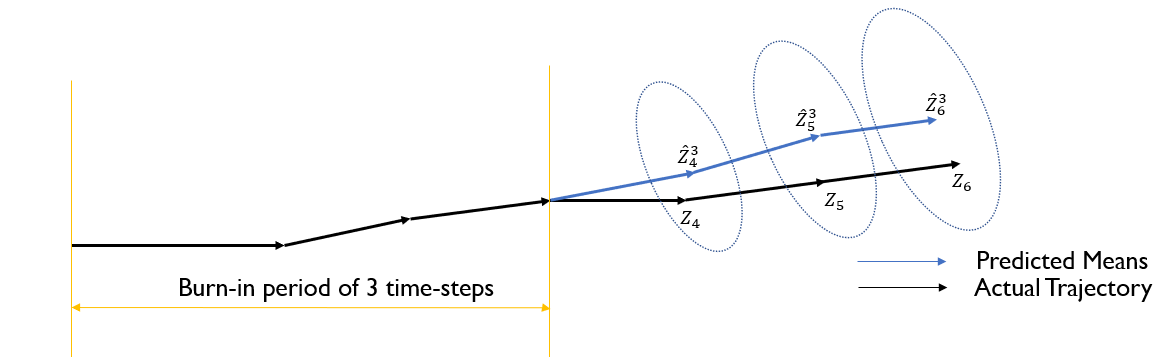
\includegraphics[scale=0.5]{method/cov_prediction.PNG}
\caption{Illustration of predicted means and covariances}
\label{fig:forward_filter}
\end{figure}

\subsection{Vanilla Long Short Term Memory networks}\label{ssec:vanilla_lstm}

There are two major limitations to using the CV model for predictions:
\begin{itemize}
    \item The transition from the hidden state at time $t$ to the hidden state at time $t+1$ is a linear transition. The emission between the hidden state and the observed state is also linear.The behaviour of road users is highly non-linear and modeling through this kind of a linear Gaussian state space model is not ideal.
    \item The number of parameters in the hidden state is very few. Usually pedestrian/cyclist behavior cannot be explained only through their past positions and speeds. For example a cyclist when executing a turn, traverses a curve and this curve is dependent on the speed he/she has when making this turn.  There are many more such behaviors and in-turn more parameters that decide trajectory of a road user
\end{itemize}

One way of solving these limitations is to resort to non-linear state space models. However, it has been seen (\cite{hutchison_pedestrian_2013}) that they don't offer considerable lift from a CV model. This is probably because even these models assume some kind of road user behavior which is not always displayed by a road user in isolation. A road user can alternate between behaviors such as constant velocity or constant acceleration or constant turn depending on the situation. Also, as the non-linear model complexity increases, it becomes increasingly difficult to use parameter estimation algorithms such as the EM algorithm as calculating closed form update equations for the parameters become increasingly complex.

Therefore, it may be necessary to move away from filter-based models and rather look at an unlikely philosophical off-shoot of the Kalman Filter. The below equation governs the mechanics of the Elman network. This network also has a hidden state propagating forward in time and an observed state which is a function of the hidden state.

\begin{equation}
\begin{split}
    h_t&=\sigma_h(W_hx_t+U_{h}h_{t-1}+b_h)\\
    y_t&=\sigma_y(W_yh_t+b_y)
\end{split}
\end{equation}

where $W_h$, $U_h$, $W_y$, $b_h$,$b_y$ represent parameter weight,bias vectors and $\sigma_h$,$\sigma_y$ represent activation functions. This is a widely used RNN-variant and improves on the Kalman Filter as all the relationships between the hidden states and the observed state is non-linear. With the help of backpropagation, all the parameter weights and biases can be obtained through training on the data. If the parameters are known, the network can be propagated forward in time to obtain estimates of $h_t$ and $y_t$. Thus these networks are more complex and at the same time easier to train, which make it a top choice for understanding patterns in temporal data. However, when the trajectory lengths are long these networks suffer from the vanishing gradient or the exploding gradient problem.  To overcome these shortcomings of an RNN, Long Short Term Memory (LSTM) was introduced. Moreover LSTM networks have also been widely used with high degrees of success in intent prediction tasks (insert references). The idea behind using an LSTM network for our problem is to better capture the dynamics of a road user's trajectory, compared to the CV model. 

The implementation of this network is done on PyTorch. The data is fed into the network in the format mentioned in Eq. \ref{eq:lstm_data}.Every neural network takes as input batches of data of size $b$. The forward step is done on the entire batch of data and this basically means that multiple tuples $input_1,input_2,...,input_b$ are clustered together and fed forward into the neural network. Each of these inputs consist of feature representations of the entire trajectory. At a particular time step $t$ a feature representation consists of the x,y coordinate as well as dummy variables indicating the type of road user. Therefore each of these inputs are of size $t \times 4$ where t signifies trajectory length. Inside a batch of data, the first input may have a trajectory length of 200, whereas the second input may have a trajectory length  of just 10. In order to train a neural network, this trajectory length must be constant throughout the batch. This is because internal computations (such as calculation of intermediate outputs in a network) are done on the entire batch together. Therefore every trajectory in the batch is appended with multiples of $[0,0,0,0]$ until they reach a length of the longest trajectory in the batch. This concept is known as padding and is quite prevalent in dealing with varying length sequences. $b\times t_{max} \times 4$ is the dimension of the input data.   However, more computations are performed over these padded indices and this costs quite a lot of computation time. In order to save compute time and not make the network calculate over these padded indices, there is a very clever idea called as packing implemented in PyTorch. Let us say that there were varying length trajectories in one batch. If the lengths of these trajectories were passed as input, internally the trajectories would be sorted and stacked like the image below. 

\begin{figure}[H]
\centering
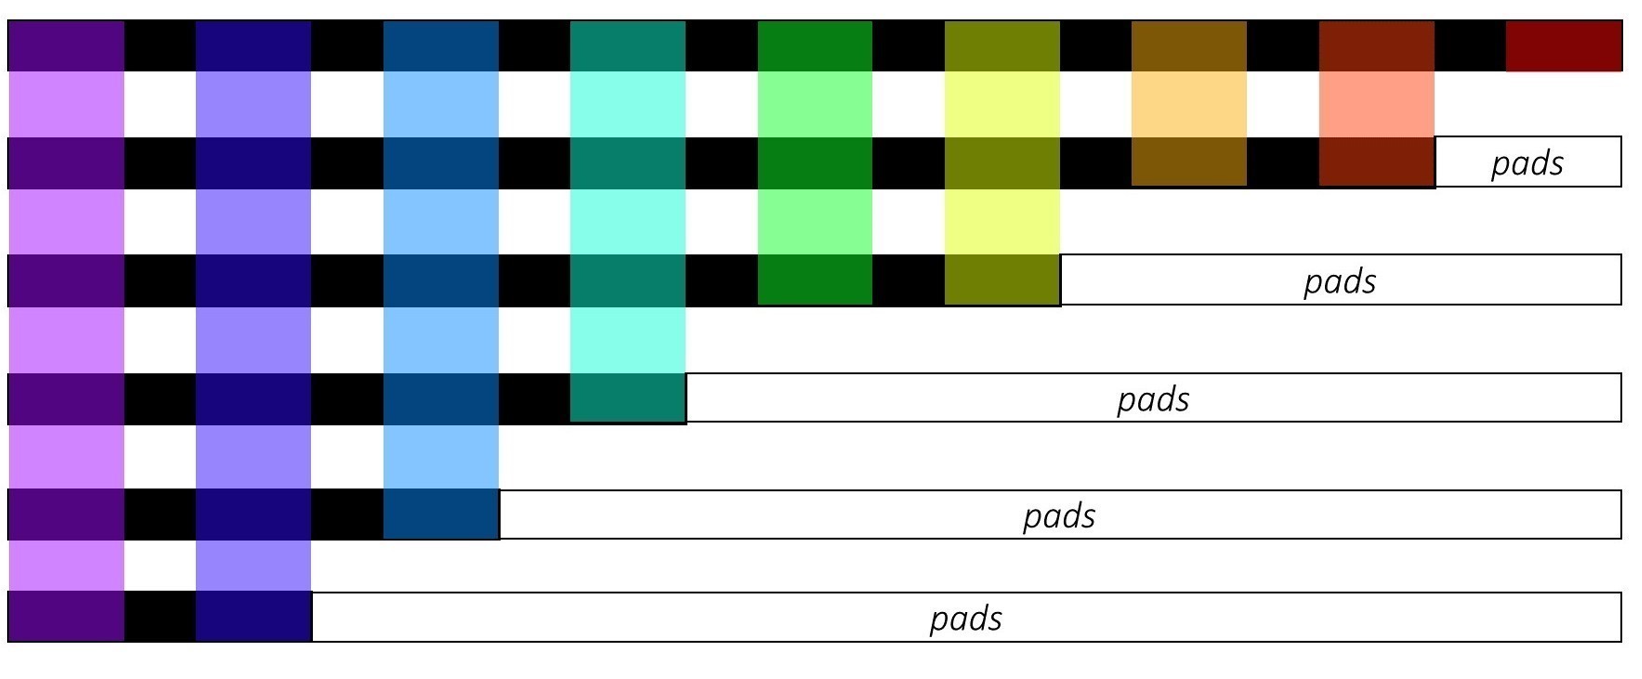
\includegraphics[scale=0.2]{method/pads.png}
\caption{Padded sequences sorted by decreasing lengths}
\end{figure}



At time step 1 and 2, the effective batch size that is considered by the network for computation is 6. This means that all the 6 observations are used for calculation of internal states. At the third time step, the effective batch size is now 5, indicating to the network that the compute now needs to be performed only for the first five observations in the entire batch. Thus, by using this concept of an effective batch size at each time step, the network knows how to ignore padded values.

For a trajectory length of $t$, the network produces the hidden states at each time step $h_1,h_2...h_t$ of size $h$ for an LSTM cell. The final hidden state $h_t$ can be considered as a good representation of the trajectory as it contains information from previous time steps. Multiple such LSTM cells can be stacked one after the other so that the output of one LSTM cell is the input to another. If there are $n$ layers, then $n$ final hidden states are obtained in total ($h_t^1,h_t^2,...,h_t^n$). All of these final hidden states are concatenated to obtain a total dimension of $nh$. This concatenated hidden state is then finally passed through a feedforward layer which brings down the dimensions required such that for each trajectory, the output from the LSTM and feedforward layer is $k$-dimensional.

\begin{figure}[H]
\centering
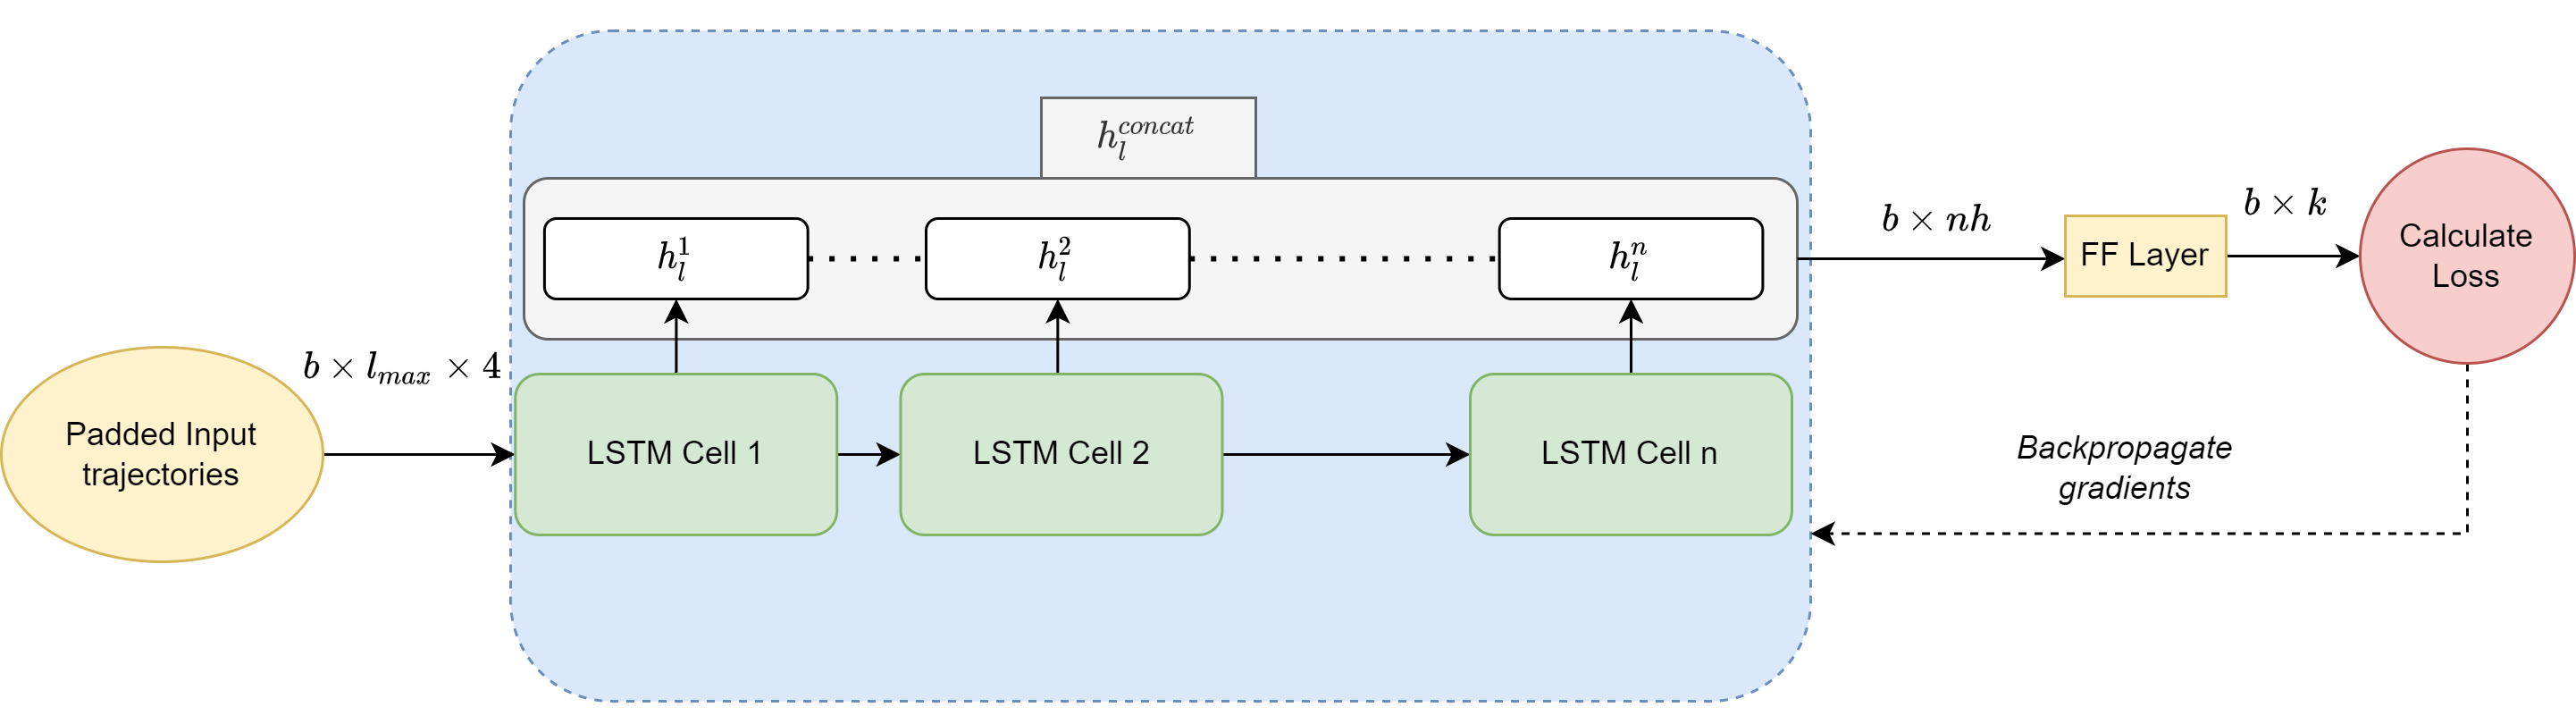
\includegraphics[scale=0.2]{method/lstm.png}
\caption{The architecture of the Vanilla LSTM approach}
\end{figure}

 $h,n$ are the hidden layer size and the number of hidden layers and these are design choices that are made to tune the network's performance. In addition $k$ can be chosen to represent two different kinds of predictions:
 \begin{itemize}
     \item The final predictions can be made to represent the  x and y coordinate of the road user at time step $t+s$. 
    \begin{equation}
    MSE=\frac{\sum_{t=1}^n(x_t-\hat{x}_t)^2+(y_t-\hat{y}_t)^2}{n}
    \end{equation}
    Mean Squared Error can be used as a loss function which needs to be minimized. An alternative metric that can be measured is the average final displacement error (AFDE), which is the displacement between the final predicted and actual position. This is computed as follows:
    \begin{equation}
    AFDE=\frac{\sum_{t=1}^n\sqrt{(x_t-\hat{x}_t)^2+(y_t-\hat{y}_t)^2}}{n}
    \end{equation}
    In our case, MSE is used as the loss function. For every batch, MSE is computed and the gradients for this loss are back-propagated through the network to obtain an update for each parameter in the network. In this case, the feedforward layer brings down the dimension coming out of the LSTM output to 2. 
    \item 
Instead of directly predicting the positions, one can also predict the means and covariances of a normal distribution such that 
\begin{equation}
    (\hat{x_t},\hat{y_t})\sim N(\mu_t,\sigma_t,\rho_t)
\end{equation}
where $\mu_t,\sigma_t,\rho_t$ represent the predicted means, covariances and correlation coefficient. The log-likelihood of observing $(x_t,y_t)$ given this normal distribution can be written as 
\begin{equation}\label{eq:lloss}
\begin{split}
    log (p(x_t,y_t |\mu_t,\sigma_t,\rho_t ))&=\log (N(\mu_t,\sigma_t,\rho_t ))\\
    &=\log N(\begin{pmatrix}
    \mu_{t,x}\\
    \mu_{t,y}
    \end{pmatrix},
    \begin{pmatrix}
    \sigma^2_{t,x} & \rho_t\sigma_{t,x}\sigma_{t,y}\\
    \rho_t\sigma_{t,x}\sigma_{t,y} & \sigma^2_{t,y}\\
    \end{pmatrix}
    )
\end{split}
\end{equation}

where $\mu_{t,x},\mu_{t,y}, \sigma_{t,x}, \sigma_{t,y}, \rho_t$ represent the predicted x and y-coordinate means, their respective variances and also the correlation coefficient
The objective is to now maximize the log-likelihood in \ref{eq:lloss} and it can analytically be shown for that for a bivariate normal distribution,maximizing the log-likelihood is equivalent to minimizing $f(x,y,\mu_{t,x},\mu_{t,y}, \sigma_{t,x}, \sigma_{t,y}, \rho_t)$ where $f$ is given in the below equation. 

\begin{equation}\label{eq:lloss_minimize}
\begin{split}
    f(x,y,\mu_{t,x},\mu_{t,y}, \sigma_{t,x}, \sigma_{t,y}, \rho_t)&=    \log(\sigma_{t,x}\sigma_{t,y})+0.5[\log(1-\rho_t^2)]+0.5(x_t-\mu_{t,x})^2\sigma_{t,y}^2\\ &+0.5(y_t-\mu_{t,y})^2\sigma_{t,x}^2 -\rho_t(y_t-\mu_{t,y})(x_t-\mu_{t,x})\sigma_{t,x}\sigma_{t,y}
\end{split}
\end{equation}

Instead of the network predicting $\sigma_{t,x}, \sigma_{t,y}, \rho_t$, the network can instead be made to predict $\log(\sigma_{t,x}), \log(\sigma_{t,y})$ and $\arctanh(\rho_t))$ for numerical stability. In addition to $\mu_{t,x}$ and $\mu_{t,y}$ the network predicts a 5-dimensional output. Hence the feedforward layer in this case brings down the dimension coming out of the LSTM output to 5. 
 \end{itemize}



\subsection{Attention based LSTM network}\label{ssec:tlstm}
There is one limitation to the approach used in the above section. The Vanilla LSTM model tries to model the dynamics of individual trajectories in the best way possible. However, sometimes road user dynamics are also governed by some other road user in the vicinity. For example, if there was a cyclist coming in front of a pedestrian, either of them will move away from the point of collission. Also, there are cases when two pedestrians moving in the same direction move similarly as one follows the path that the other has taken subconsciously. Road users tend to make these complex maneuvers that takes into consideration other road users without seemingly thinking a lot about it. Therefore, when it comes to predictions, it becomes important to incorporate the social aspect of behaviors in a road user's trajectory. The Social-LSTM \cite{alahi_social_2016} is a recent state-of-the-art model that has shown to capture these social interactions to a reasonable extent. The principle of a social LSTM is to combine the workings of a Vanilla LSTM with a so-called social pooling layer. At a particular frame, all road users' features are passed into a plain LSTM network. This LSTM network then produces hidden states for each of these road users. These hidden states represent what a road user would do without the presence of other social factors.  If a pedestrian's trajectory needs to be predicted, then their neighbors' (who are within a certain spatial distance) hidden states are stacked in a specific way to construct a pooled tensor (will be added in the relevant literature section). In our method instead of using this pooling, an attention mechanism is used to capture how much attention each road user gives each other. Therefore the output representation coming from the LSTM network for each road user is then passed through an attention layer. The hypothesis for building this kind of a network is that:
\begin{itemize}
    \item The LSTM networks should output a representation of a road user's behavior without any social influence
    \item If a road user's trajectory was changed due to some other road user(s) in the network, this behavior should be captured by the attention layer 
\end{itemize}

Practically, this is implemented as a transformer encoder architecture which basically consists of multi-head attention layer and a feedforward layer as mentioned in Section \ref{ssec:transformers_theory} .
The format of data that is passed into the network is mentioned in Eq. \ref{eq:transformers_data}. Essentially, the number of road users in a frame is another dimension that is added to the previous data used for the Vanilla LSTM network. The input to the vanilla LSTM network was of dimensions $b \times l_{max} \times 4$. The output coming from the LSTM network for each road user is of dimension $b \times nh$ where $h$ is the dimension of the hidden state. In total there will be $r$ hidden states for all road users present in the frame. In a batch of frames, there may be instance with different number of road users in each frame. A network cannot take variable sized input and therefore one option is to pad the hidden states outputted from the LSTM network and then pass it into the transformer. However, the idea of packing cannot be used in a transformer as a transformer computes on all instances of time at once. There is no recurrent nature in a transformer and because of this, the concept of effective batch size cannot be used. One solution is to use the concept of attention masking where attention scores are not calculated for padded positions in the input. The concept used in this thesis is to batch together all frames/instances where the number of road users are same. For example there may be multiple instances/occurrences when there are 4 road users in a frame. All these instances are batched together and sent into the Attention based LSTM network. The number of road users in a frame can range between 0 to 20. Again, a feedforward network is used to bring down the dimension of the output coming from a transformer. The final predictions are made for all the road users in the frame and thus the loss for every training instance can be the MSE loss or the log-likelihood loss presented in the previous section. In the case that the road user has exited the frame at prediction time, the actual positions of the road user is unknown. In these  circumstances, loss is not calculated for these road users. 

\begin{figure}[H]
\centering
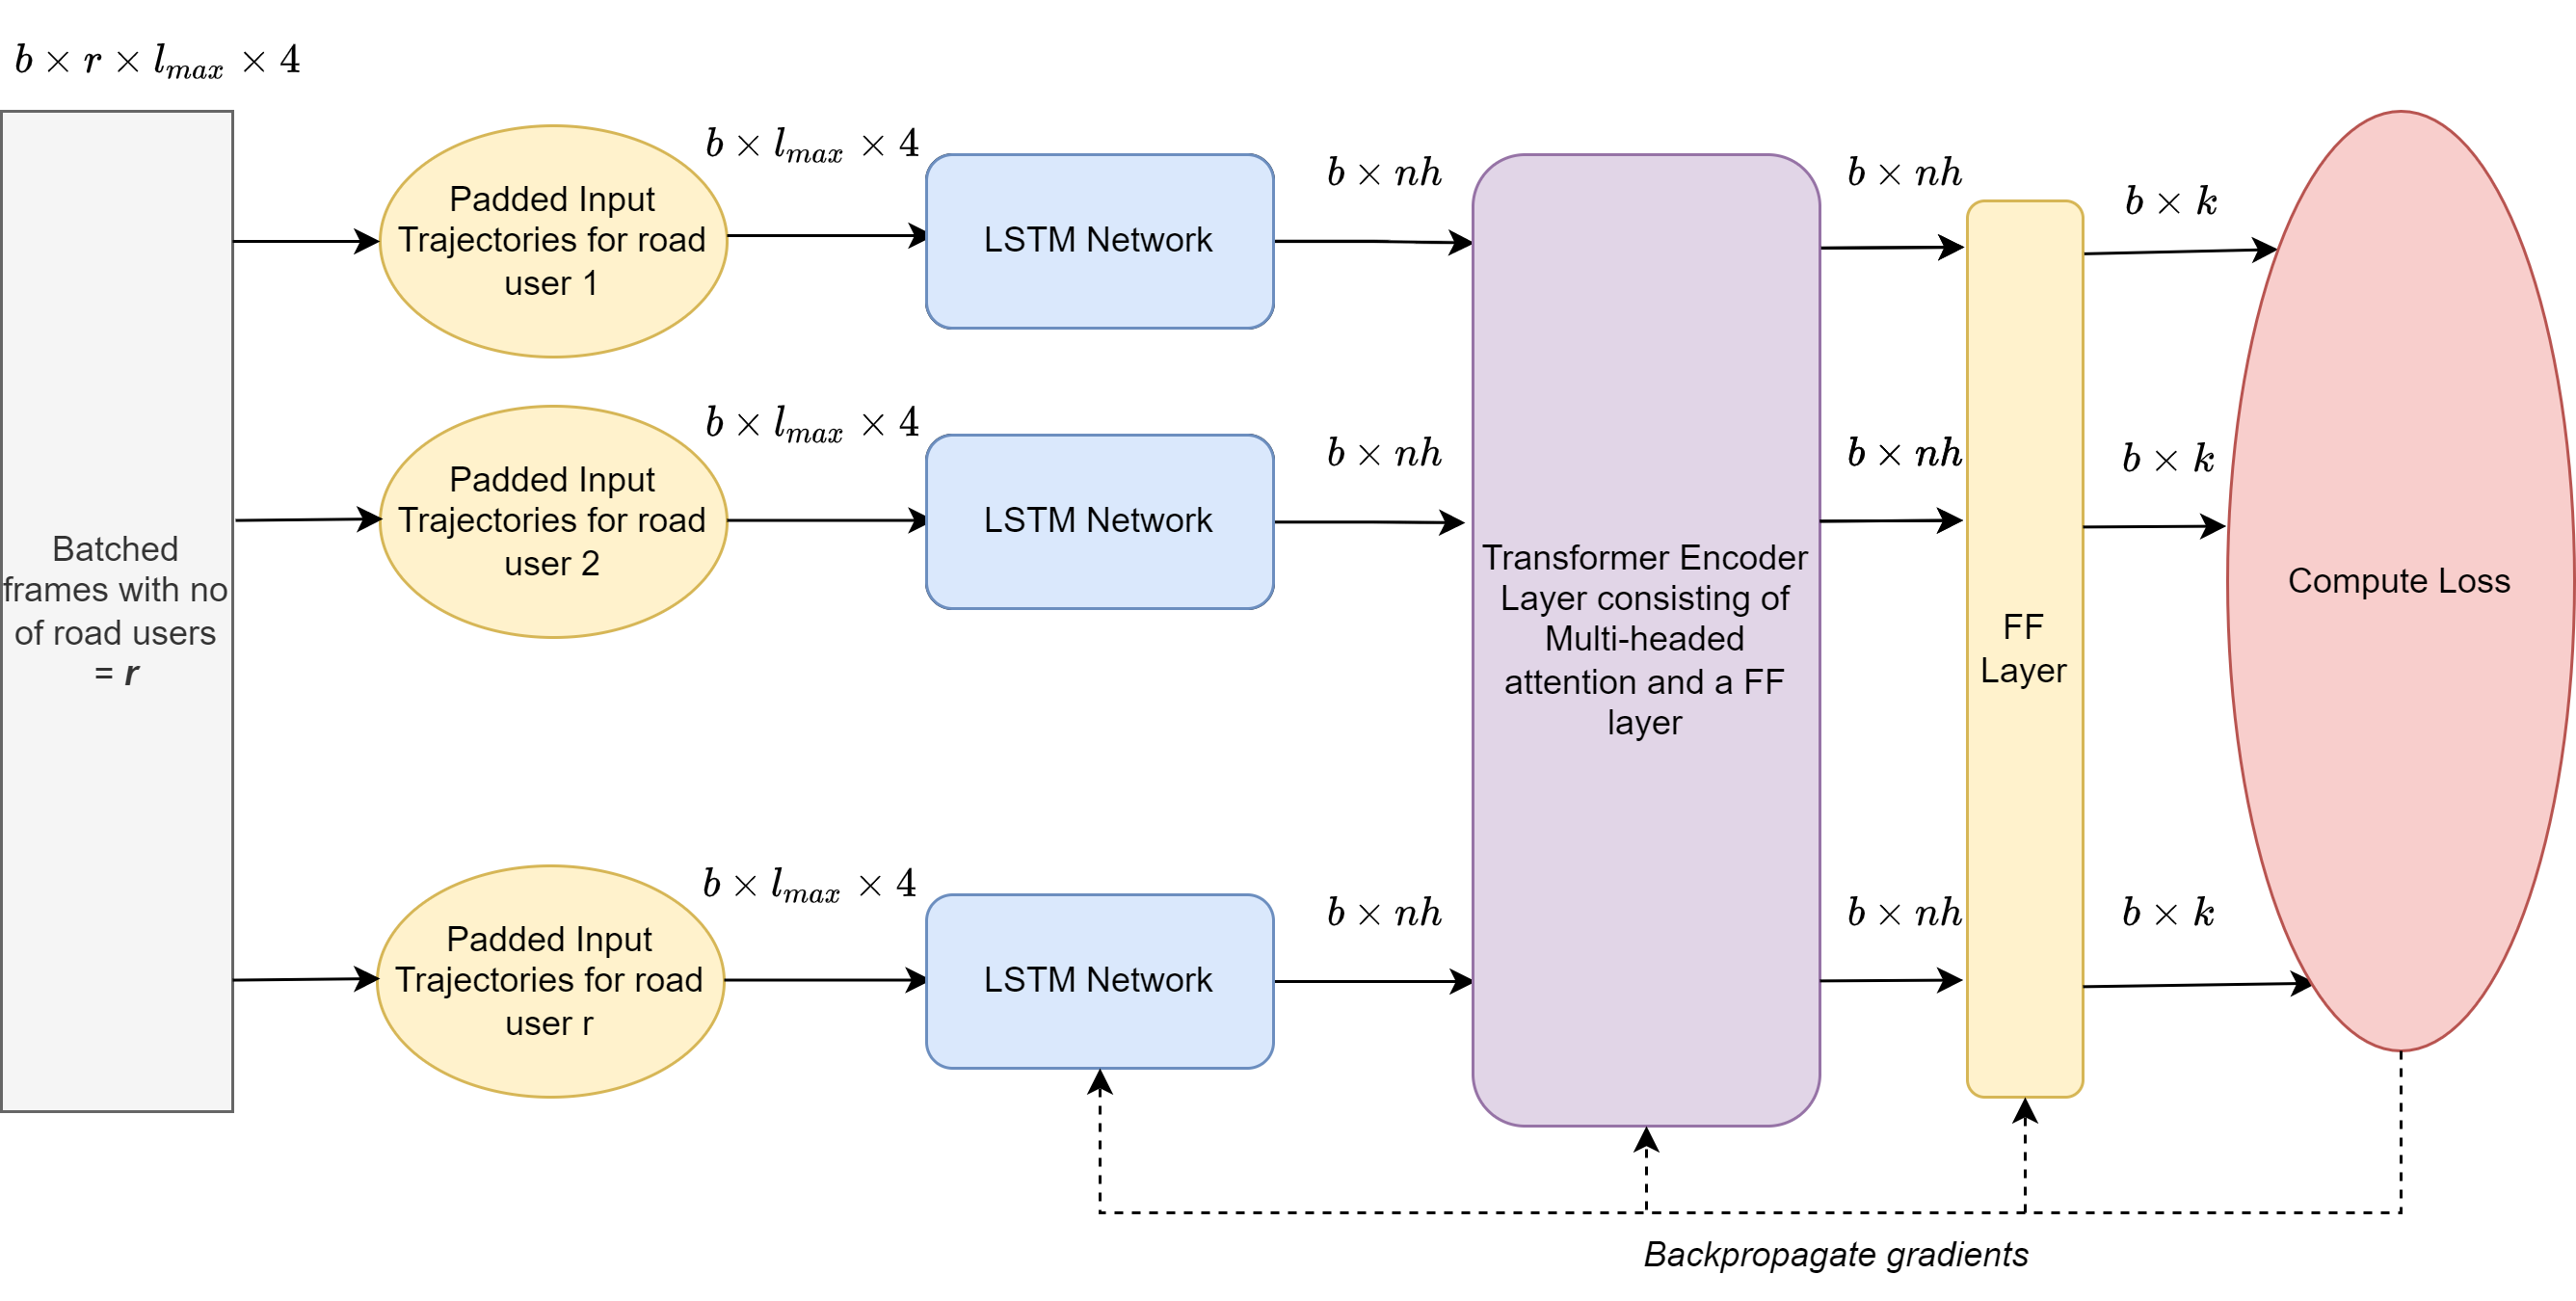
\includegraphics[scale=0.15]{method/tlstm.png}
\caption{Architecture of the self-attention based LSTM}
\end{figure}



\section{Results and Discussion}
In this section, we will focus on the quantitative and qualitative results obtained through applying the various methods on our data. Firstly there are two datasets: the dataset with a sampling time of $0.2$ seconds and a dataset with sampling time $1$ second. For convenience we will call them dataset 1 and dataset 2 respectively. The Kalman Filter constant velocity model has been trained and tested on both these datasets, whereas the neural network models have been trained and tested on dataset 2. This is because it is computationally more expensive to train the network on the dataset 1, as there are 5 times the number of observations. The chosen dataset is then split into train/test/validation. Since this data was collected over a week, 4 days of this week including a weekend have been chosen for training. 2 days (including another weekend) of data have been used for testing with the remaining 1 day used for validation. Also, for the purposes of training, a minimum of 2 seconds of past trajectory is required as mentioned in the data exclusions section. This means that all trajectories are at least 2 seconds old. Given trajectories up till time $t$, the prediction task is to approximate the position of the road user $s$ steps ahead. If $s$ is chosen to $<$ 1 second, the prediction although accurate won't be helpful since all reactions to this prediction should be made in less than 1 second and this isn't practically possible. If $s$ is chosen to be very high (say $>$ 6 seconds), the predictions themselves will deviate a lot from the actual positions, since there is high scope for change in trajectory with such a large window. Therefore it was decided to predict 3 seconds into the future and this setting applies to all the results mentioned here. 

\subsection{Constant Velocity Model}
For this model, the train/test/validation split was done on dataset 1 and dataset 2. \ref{alg:em} was used on the training data to obtain parameter estimates for $Q$, $R$. It was seen that these matrices converged in 10-15 iterations/passes through the data. The obtained parameters were then used to propagate the model forward and obtain the mean and covariance of prediction. The below table tabulates the mean squared error on the test,validation dataset for the three different road users. 

\begin{table}[H]
\parbox{.45\linewidth}{
\centering
\begin{tabular}{@{}cccc@{}}
\toprule
Road User & 0.2s Dataset & 1s Dataset \\ \midrule
Pedestrian  & 1.4 & 1.2 \\ 
Cyclist  & 2.8 & 3.7 \\
Shuttle  & 2.4 & 2.4 \\  \midrule
Total & 1.9 & 2.2 \\    \midrule
%\bottomrule
\end{tabular}
\caption{Mean Squared Error on test}
\label{table:1}
}
\hfill
\parbox{.45\linewidth}{
\centering
\begin{tabular}{@{}cccc@{}}
\toprule
Road User & 0.2s Dataset & 1s Dataset \\ \midrule
Pedestrian  & 1.2 & 1.2 \\ 
Cyclist  & 2.7 & 3.6 \\
Shuttle  & 1.7 & 1.2 \\  \midrule
Total & 1.8 & 2.2 \\    \midrule
%\bottomrule
\end{tabular}
\caption{Mean Squared Error on validation}
\label{table:2}
}
\end{table}
Apart from MSE, the likelihood of observing the actual position given the predicted mean and covariance can be estimated. The average log-likelihood estimate can be constructed as below:
\begin{equation}
    \frac{\sum_{i=1}^n\sum_{t=1}^{t_i}\log(p(x_t,y_t)|\mu_{x,t},\mu_{y,t},\Sigma_t)}{\sum_{i=1}^n\sum_{t=1}^{t_i}[\mathbbm{1}]}
\end{equation}
\\
\\

\begin{table}[H]
\parbox{.45\linewidth}{
\centering
\begin{tabular}{@{}cccc@{}}
\toprule
Road User & 0.2s Dataset & 1s Dataset 2 \\ \midrule
Pedestrian  -3.3  & -2.3 \\ 
Cyclist  & -3.8 & -3.4 \\
Shuttle  & -3.4 & -2.7 \\  \midrule
Total & -3.5 & -2.7 \\    \midrule
%\bottomrule
\end{tabular}
\caption{Avg log-likelihood on test}
\label{table:3}
}
\hfill
\parbox{.5\linewidth}{
\centering
\begin{tabular}{@{}cccc@{}}
\toprule
Road User & 0.2s Dataset & 1s Dataset  \\ \midrule
Pedestrian  & -3.3 & -2.3 \\ 
Cyclist  & -3.8 & -3.4 \\
Shuttle  & -3.4 & -2.4 \\  \midrule
Total & -3.5 & -2.7 \\    \midrule
%\bottomrule
\end{tabular}
\caption{Avg log-likelihood on validation}
\label{table:4}
}
\end{table}

As can be seen from Tables \ref{table:1} \ref{table:2}, the MSE is almost similar for all road users except for cyclists where MSE is lower for the 0.2s dataset. This is because cyclists tend to move faster and a higher sampling time will give relatively more information. Also Tables \ref{table:3} \ref{table:4} present the average log-likelihood score. This score cannot be compared across the two differently sampled datasets, as the distributions are different. Both distributions have different covariance matrices and hence differently shaped distributions. The probability of observing the same point with respect to both these distributions will be different. 
\subsection{Hyperparameter-tuning}
\subsubsection{Vanilla LSTM}
For the vanilla-LSTM, the number of layers and the size of hidden layers are two important hyperparameters. To tune them, a coarse grid hyperparameter tuning was performed where the different networks were trained on different parameters. The networks' test and validation MSE is shown below:
% Please add the following required packages to your document preamble:
% \usepackage{booktabs}
% \usepackage{multirow}
% \usepackage[table,xcdraw]{xcolor}
% If you use beamer only pass "xcolor=table" option, i.e. \documentclass[xcolor=table]{beamer}
\begin{table}[H]
\centering
\begin{tabular}{@{}ccc@{}}
\toprule
\multicolumn{1}{l}{Hidden Layer Size} & \multicolumn{1}{l}{Number of  LSTM layers} & \multicolumn{1}{l}{Validation MSE} \\ \midrule
                                      & 2                                          & 1.18                               \\
                                      & 3                                          & 1.16                               \\
\multirow{-3}{*}{10}                  & 4                                          & 1.16                               \\ \midrule
                                      & 2                                          & 1.13                               \\
                                      & 3                                          & 1.13                               \\
\multirow{-3}{*}{16}                  & 4                                          & 1.10                               \\ \midrule
                                      & 2                                          & 1.09                               \\
                                      & 3                                          & 1.12                               \\
\multirow{-3}{*}{20}                  & 4                                          & 1.09                               \\ \midrule
                                      & 2                                          & 1.08                               \\
                                      & 3                                          & 1.09                               \\
\multirow{-3}{*}{25}                  & 4                                          & 1.07                               \\ \midrule
                                      & 2                                          & \cellcolor[HTML]{32CB00}1.05       \\
                                      & 3                                          & 1.05                               \\
\multirow{-3}{*}{28}                  & 4                                          & 1.05                               \\ \bottomrule
\end{tabular}
\end{table}

As can seen from the figure above, the test MSE is very similar for the last three entries and the least complex network was chosen (highlighted in green)
\subsubsection{Self Attention based LSTM}
To train this network, parameters were shared from the trained LSTM network and a similar cross-validation was performed, with an additional parameter of number of attention heads.
\begin{figure}[H]
\centering
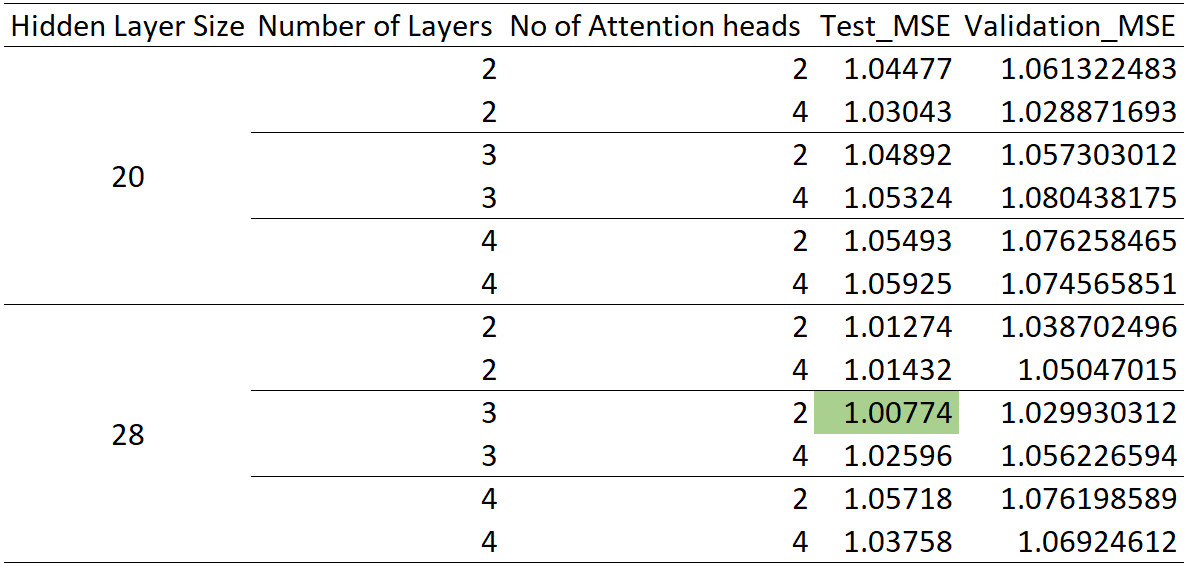
\includegraphics[scale=0.5]{result/res2.png}
\caption{Hyperparameter tuning for the Self Attention based LSTM network}
\end{figure}

\subsection{Analyzing and comparing the different methods}
The best models were chosen through hyperparameter tuning and the MSE obtained for different road users is tabulated below:
\begin{figure}[H]
\centering
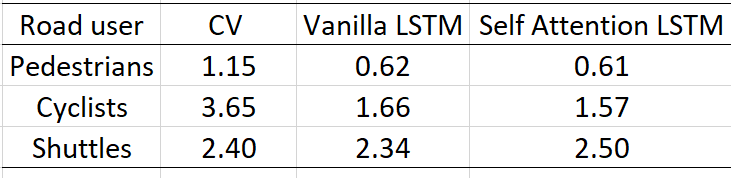
\includegraphics[scale=0.6]{result/res3.png}
\caption{Comparison of different models on different road users}
\end{figure}
Also, the hypothesis is that the self-attention model fares better than the Vanilla LSTM model when the number road users increase. To test this, we have plotted MSE against the number of road users and also taken a ratio of errors between the attention based vs plain architecture. 
\begin{figure}[H]
\centering
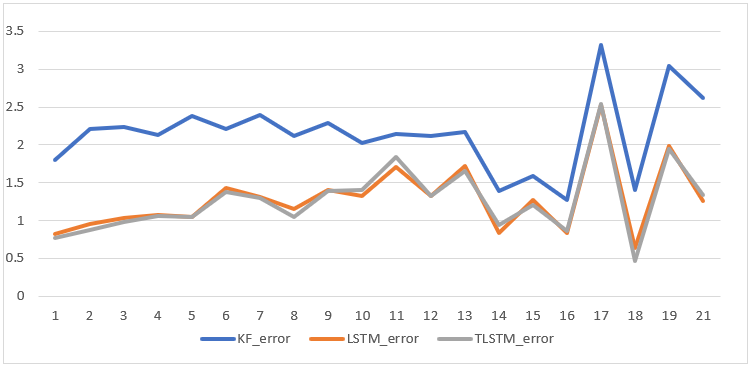
\includegraphics[scale=0.6]{result/res4.png}
\caption{MSE for different number of road users in the scene}
\end{figure}

\begin{figure}[H]
\centering
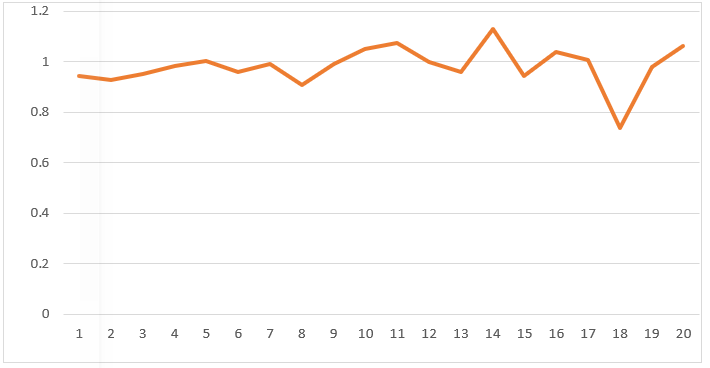
\includegraphics[scale=0.6]{result/res5.png}
\caption{Ratio of MSE between the Attention based vs Vanilla architecture}
\end{figure}

\subsection{Qualitative Analysis}
The above section dealt with quantitatively comparing different models. It would also be interesting to assess the behaviors that these models try to capture. Therefore this section is dedicated to visualizing predictions made by these models, in an attempt to delineate these models better.

\begin{figure}[H]
\centering
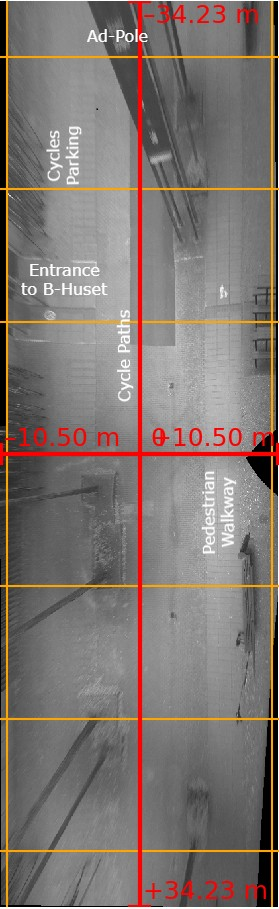
\includegraphics[scale=0.3]{quali_results/ground.jpg}
\caption{Map of the ground frame}
\end{figure}


For convenience, in all the figures above the vertical axis is called as the y-axis and the horizontal axis is called as the x-axis. Pedestrians and cyclists usually move longitudinally along the y-axis and in some instance take turns or slight maneuvers so that their x-coordinate also changes. Along the left end of the image there is an entrance to the building and cycles are parked along the left border of the image. 

\begin{figure}[H]
\centering
\begin{subfigure}{0.5\textwidth}
  \centering
  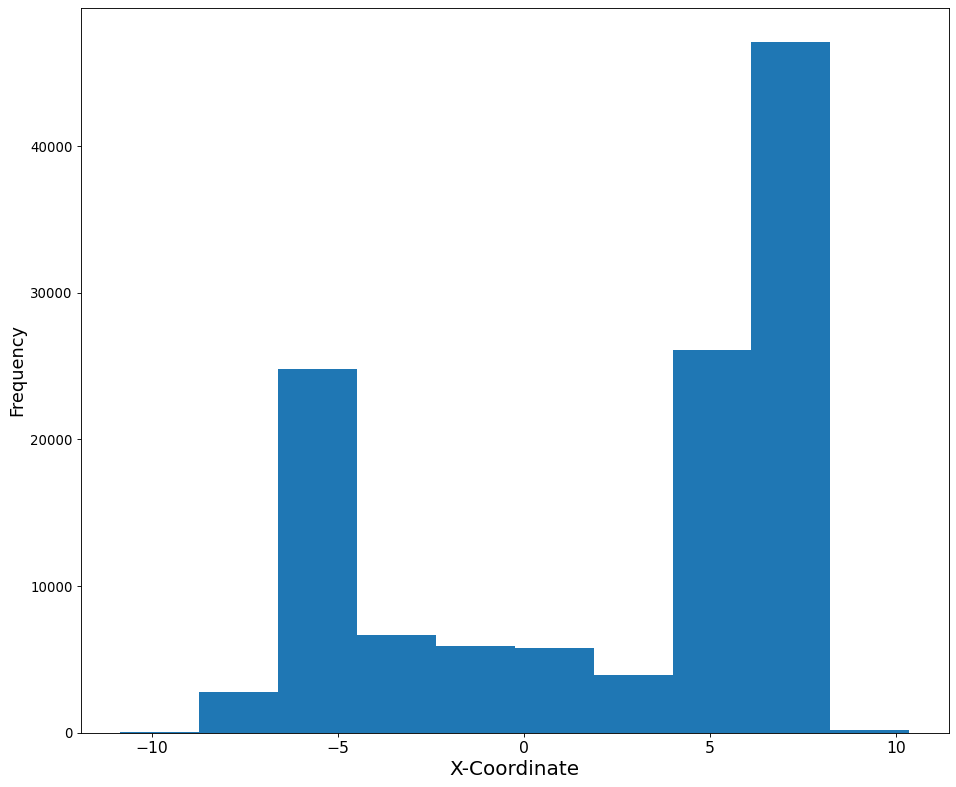
\includegraphics[width=\linewidth]{quali_results/hist-ped.png}
  \caption{Pedestrians}
  \label{fig:cyc-1-1}
\end{subfigure}%
\begin{subfigure}{0.5\textwidth}
  \centering
  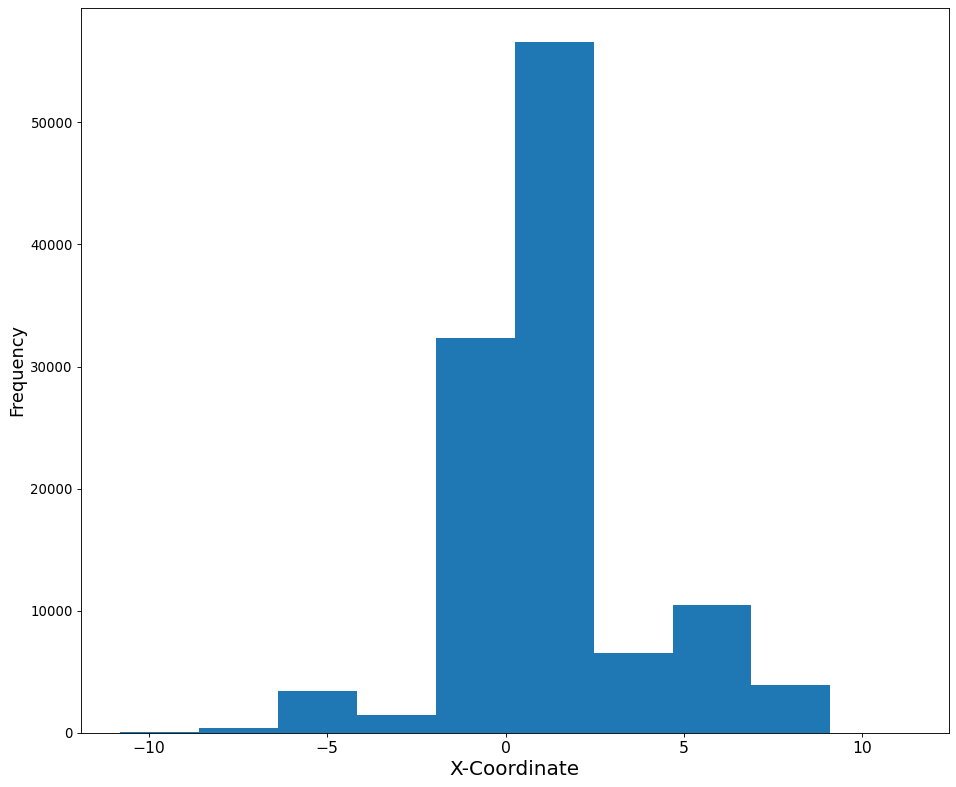
\includegraphics[width=\linewidth]{quali_results/hist-cycle.png}
  \caption{Cyclists}
  \label{fig:cyc-1-2}
\end{subfigure}
\caption{Distribution of x-coordinates for road users}
\label{fig:cyc-1}
\end{figure}

As seen in the above image, cyclists generally  move closer to the center of the axis. Pedestrians usually traverse on the ends of the frame, specifically on the right as there is a pedestrian walkway present there. 


In all the figures from here on, the solid black line represents the past trajectory, the dotted-line represents the future trajectory. In some images, an arrow will be showcased to illustrate the start position and direction of the road user.  The blue, green and red crosses represents the 3-step ahead prediction for the constant velocity model, vanilla LSTM network (referred to as the LSTM network) and the Transformer/Attention based LSTM network (for convenience this is called as the TLSTM network). For conveniences,each of these trajectories are also labelled with the type of road user (Cyclist, Pedestrian, Shuttle) and a unique ID (1,2,3..) for each road user to isolate and differentiate trajectories. Also the frame number added to the images indicate the moment from which predictions are being made. Frame 1 signifies the  prediction made from the first 2 seconds of trajectory input, frame 2 signifies the prediction made the first 3 seconds of input and so on.
After individually studying many trajectories and running simulations of the videos, some behaviors were seen for the various models on the given data. It is to be pointed out that the trends seen here aren't a representative trend for the entire dataset and is rather a representative from a sample. These samples were obtained by looking at entries where one model's error is lower compared to the other models, so that the behaviors captured/missed by the models are assessed. 

\subsubsection{CV model vs LSTM based models}
There are quite a few instances where the Constant Velocity models are not able to capture behaviors that are captured well by the LSTM based models. The first of these instances is when the constant velocity model is not able to capture self-corrections made by pedestrians and cyclists alike. This is when a pedestrian/cyclist is correcting his/her course, so that their trajectory is not obtuse and is parallel to one of the axes.

\begin{figure}[H]
\centering
\begin{subfigure}{0.4\textwidth}
  \centering
  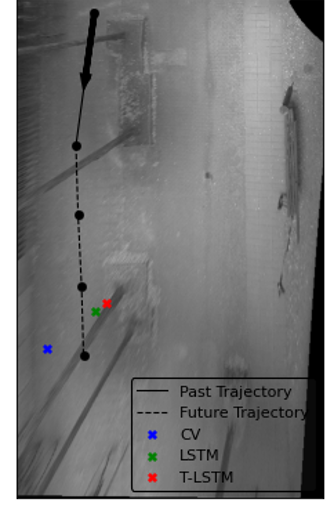
\includegraphics[width=\linewidth]{quali_results/cyc-0-1.png}
  \caption{Cyclist 0 -Frame 1}
  \label{fig:cyc0-1}
\end{subfigure}
\begin{subfigure}{0.4\textwidth}
  \centering
  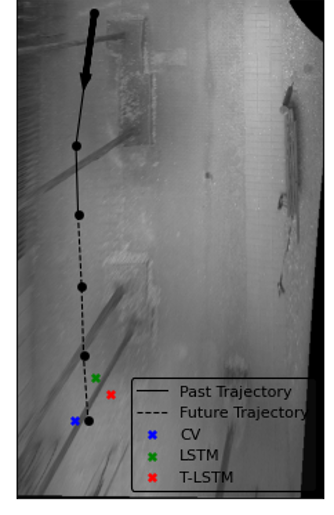
\includegraphics[width=\linewidth]{quali_results/cyc-0-2.png}
  \caption{Cyclist 0 - Frame 2}
  \label{fig:cyc0-2}
\end{subfigure}
\begin{subfigure}{0.40\textwidth}
  \centering
  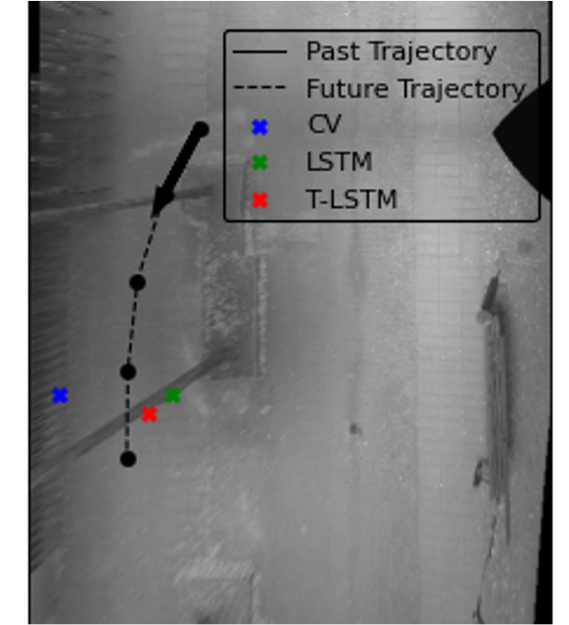
\includegraphics[width=\linewidth]{quali_results/first-1.png}
  \caption{Cyclist 1 Frame 1}
  \label{fig:cyc1-1}
\end{subfigure}
\begin{subfigure}{0.40\textwidth}
  \centering
  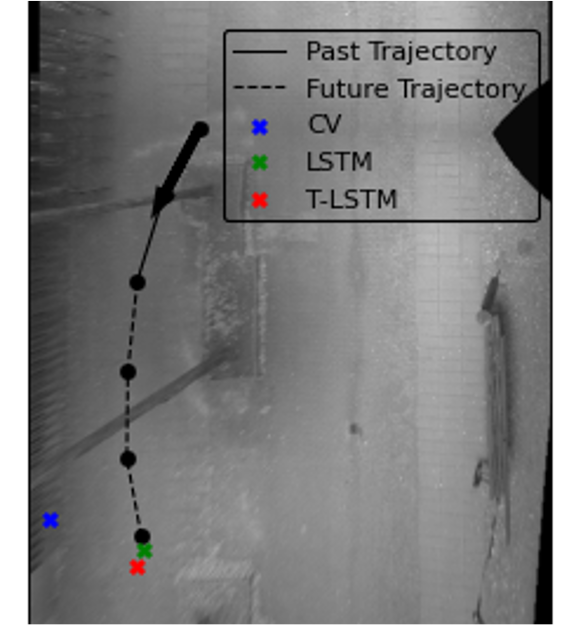
\includegraphics[width=\linewidth]{quali_results/first-2.png}
  \caption{Cyclist 1 Frame 2}
  \label{fig:cyc1-2}
\end{subfigure}
\caption{Course correction trajectories for road users }
\label{fig:cyc1&2}
\end{figure}

As can be seen from Fig. \ref{fig:cyc1&2} usually pedestrians and cyclists tend to correct their course, so that they move parallel to the y-axis. This kind of behavior is not captured by a CV model as they tend to just extrapolate current state dynamics forward in time and don't recognize such spatial dependencies. This maneuver was frequently exhibited by pedestrians and cyclists alike and was well captured by the LSTM based networks. 

Another kind of maneuver observed in the dataset is a turn. A turn can be defined as a sharp change in direction of a road user. The self-corrections that were discussed above were acute changes in direction (this can be heuristically defined as $<60^{\circ}$). A turn is an obtuse/significant change in direction ($>60^{\circ}$). These turns are hard for even human observers to detect and now we will be looking at cases where the LSTM based models are able to detect turns that were otherwise undetected by the CV model. 

\begin{figure}[H]
\centering
\begin{subfigure}{0.4\textwidth}
  \centering
  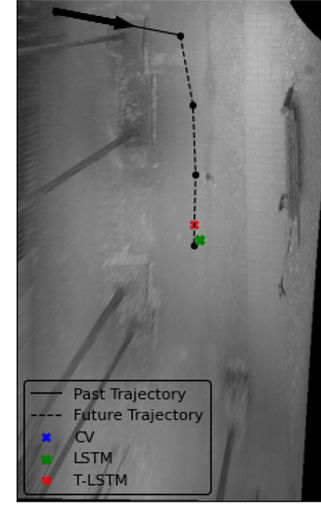
\includegraphics[width=\linewidth]{quali_results/cyc-3-1.png}
  \caption{Cyclist 2 -Frame 1}
  \label{fig:cyc2-1}
\end{subfigure}
\begin{subfigure}{0.4\textwidth}
  \centering
  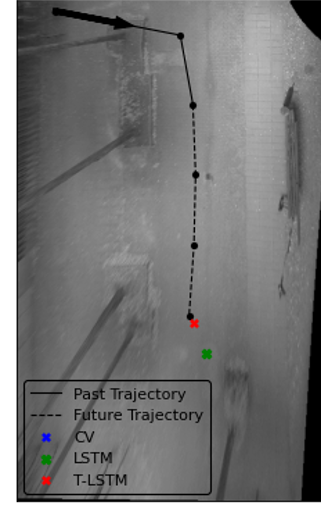
\includegraphics[width=\linewidth]{quali_results/cyc-3-2.png}
  \caption{Cyclist 2 - Frame 2}
  \label{fig:cyc2-2}
\end{subfigure}
\begin{subfigure}{0.4\textwidth}
  \centering
  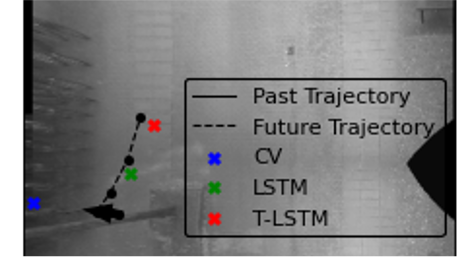
\includegraphics[width=\linewidth]{quali_results/cyc-4-1.png}
  \caption{Cyclist 3 Frame 1}
  \label{fig:cyc3-1}
\end{subfigure}
\begin{subfigure}{0.4\textwidth}
  \centering
  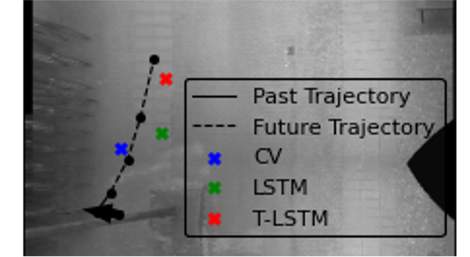
\includegraphics[width=\linewidth]{quali_results/cyc-4-2.png}
  \caption{Cyclist 3 Frame 2}
  \label{fig:cyc3-2}
\end{subfigure}
\begin{subfigure}{0.4\textwidth}
  \centering
  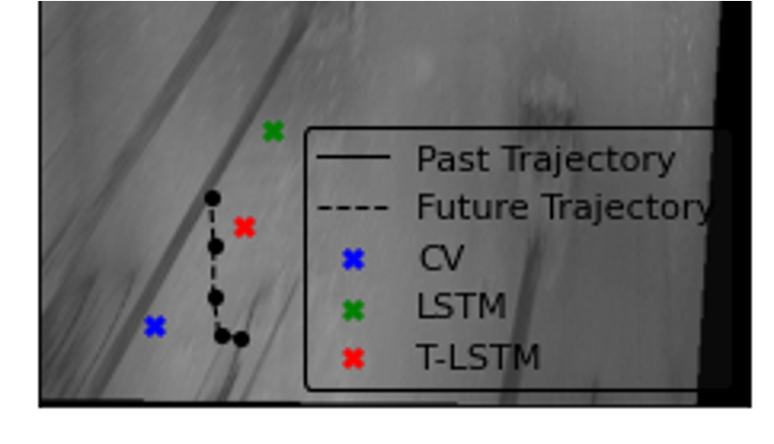
\includegraphics[width=\linewidth]{quali_results/cyc-2-1.png}
  \caption{Cyclist 4 -Frame 1}
  \label{fig:cyc4-1}
\end{subfigure}
\begin{subfigure}{0.4\textwidth}
  \centering
  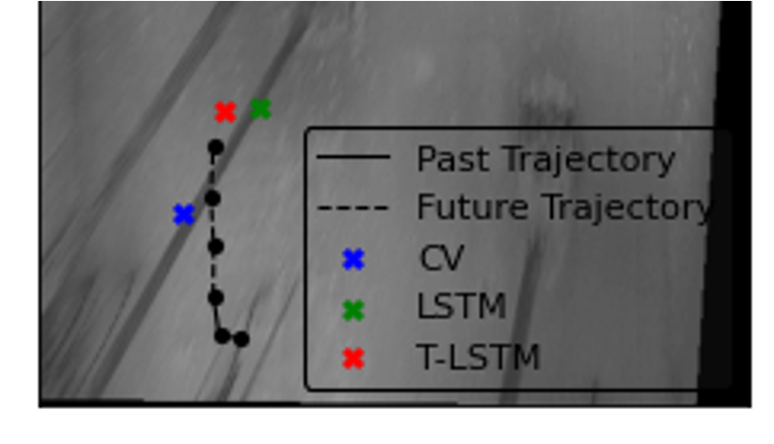
\includegraphics[width=\linewidth]{quali_results/cyc-2-2.png}
  \caption{Cyclist 4 - Frame 2}
  \label{fig:cyc4-2}
\end{subfigure}
\caption{Turning maneuvers exhibited by road users}
\label{fig:cyc}
\end{figure}
In Fig \ref{fig:cyc2-1} and Fig. \ref{fig:cyc2-2} , the cyclist takes a turn toward the right, which has been correctly predicted by the LSTM based networks. The network would have assessed that the road user needs to correct his/her trajectory.  The movement of the cyclist towards the negative y-axis in the first two seconds may have indicated to the network that the cyclist will turn right. Figures \ref{fig:cyc3-1} \ref{fig:cyc3-2} \ref{fig:cyc4-1} and \ref{fig:cyc4-2} on the other hand are more complicated turns. These turns are perpendicular or even obtuse. There is a hint albeit slight in both these cases that the user might go towards the positive y-axis, which may be helping the network predict these turns. There are again many such cases found in the data where a turn has been correctly predicted by both the LSTM networks. 

Now, we will be looking at cases where the CV model has performed better than the two LSTM based networks. 

\begin{figure}[H]
\centering
\begin{subfigure}{0.4\textwidth}
  \centering
  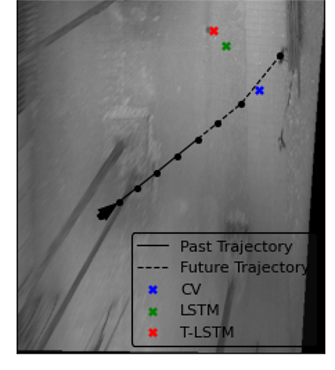
\includegraphics[width=\linewidth]{quali_results/cyc-5-1.png}
  \caption{Cyclist 5 -Frame 1}
  \label{fig:cyc5-1}
\end{subfigure}
\begin{subfigure}{0.4\textwidth}
  \centering
  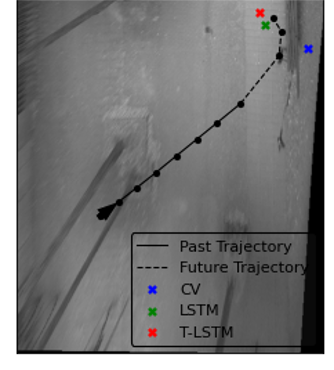
\includegraphics[width=\linewidth]{quali_results/cyc-5-2.png}
  \caption{Cyclist 5 - Frame 2}
  \label{fig:cyc5-2}
\end{subfigure}
\begin{subfigure}{0.40\textwidth}
  \centering
  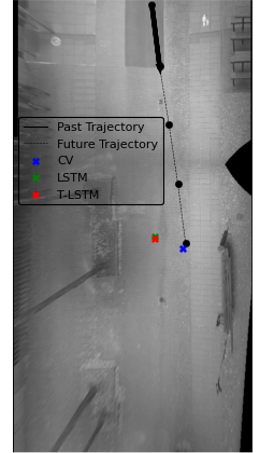
\includegraphics[width=\linewidth]{quali_results/cyc-6-1.png}
  \caption{Cyclist 6 Frame 1}
  \label{fig:cyc6-1}
\end{subfigure}
\begin{subfigure}{0.40\textwidth}
  \centering
  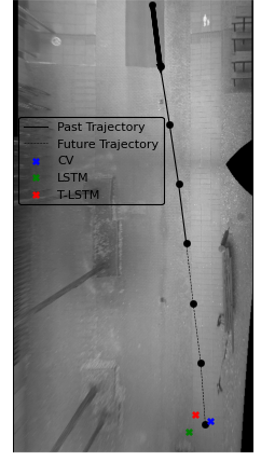
\includegraphics[width=\linewidth]{quali_results/cyc-6-2.png}
  \caption{Cyclist 6 Frame 2}
  \label{fig:cyc6-2}
\end{subfigure}
\caption{Trajectories where road users don't course correct}
\label{fig:cyc5&6}
\end{figure}

Now in these cases we notice that the road users don't course correct and these cases are unusual in the dataset. In such cases, it is noticed that the LSTM networks always try for course-correction at a suitable place and eventually as the past trajectory length gets longer in the same straight line, they go for a more conservative (and not immediate) course-correction close to the end of the frame. 


\begin{figure}[H]
\centering
\begin{subfigure}{0.39\textwidth}
  \centering
  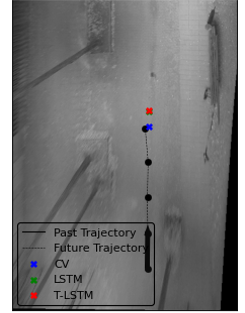
\includegraphics[width=\linewidth]{quali_results/cyc-7-speed.png}
  \caption{Cyclist 7 -Frame 1}
  \label{fig:cyc7-speed}
\end{subfigure}
\begin{subfigure}{0.39\textwidth}
  \centering
  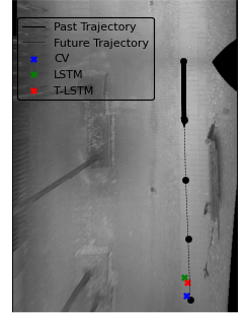
\includegraphics[width=\linewidth]{quali_results/cyc-8-speed.png}
  \caption{Cyclist 8 - Frame 1}
  \label{fig:cyc8-speed}
\end{subfigure}
\caption{Trajectories where velocities are estimated incorrectly by the LSTM based networks}
\label{fig:cyc7&8}
\end{figure}

The above figures represent some infrequent situations when the LSTM based network either overestimates or underestimates the velocity of cyclists. Cyclists usually show higher variance in their speed and as a result their velocities are hard to estimate. In the above cases, the cyclist is travelling at a constant velocity and is thus captured well by the CV model. On the other hand the LSTM based networks add some noise as they have seen just two seconds of past trajectory data. However, it has to be pointed out that these are rare occurrences and don't represent the majority of cases where the LSTM based network either capture velocity better or to the same extent as the CV  model.



\subsubsection{LSTM vs Attention based LSTM model}
In the previous section, we compared qualitatively the behavior of a CV model vs neural network based models. In this section, we will look at comparing the two LSTM models to assess the behaviors that are captured by one and not another. In addition to the legends from the previous plots, the present plots also consists of white points. These white points represent the position of other road users in the scene \textit{at the time of prediction}. This means that if the network was predicting the ego road user's position at time $t$ using trajectory information till time $t-3$, then the white points represent all other road users present at time $t$. This adds another dimension to the image and conveys how close the ego-user's actual trajectory was to some other road users. 

\begin{figure}[H]
\centering
\begin{subfigure}{0.3\textwidth}
  \centering
  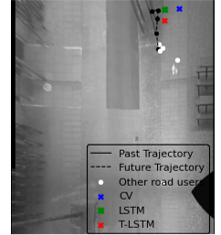
\includegraphics[width=\linewidth]{quali_results/ped-turn-1.png}
  \caption{Pedestrian 1 -Frame 1}
  \label{fig:ped-turn-1}
\end{subfigure}
\begin{subfigure}{0.3\textwidth}
  \centering
  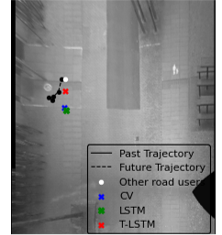
\includegraphics[width=\linewidth]{quali_results/ped-turn-2.png}
  \caption{Pedestrian 2 - Frame 1}
  \label{fig:ped-turn-2}
\end{subfigure}
\begin{subfigure}{0.3\textwidth}
  \centering
  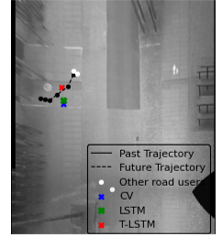
\includegraphics[width=\linewidth]{quali_results/ped-turn-3.png}
  \caption{Pedestrian 3 - Frame 1}
  \label{fig:ped-turn-3}
\end{subfigure}
\caption{Turn Trajectories correctly predicted by Attention based LSTM}
\label{fig:ped1&2&3}
\end{figure}

Figures \ref{fig:ped-turn-2} and \ref{fig:ped-turn-3} are turns at the entrance. After the first two seconds, the attention based network is correct in assessing that the pedestrian will turn left for both these cases. Another interesting observation is that this happens with other co-pedestrians as is represented from the white points. The same is the case with \ref{fig:ped-turn-1} where the pedestrian turns right. It is to be pointed out again that many pedestrians move in groups in this data. These pedestrians usually have similar trajectories and maintain a very small distance from each other. These group movement patterns may be better assessed by the Attention based LSTM networks and hence they may be able to better predict turning maneuvers exhibited by groups of pedestrians. 

\begin{figure}[H]
\centering
\begin{subfigure}{0.4\textwidth}
  \centering
  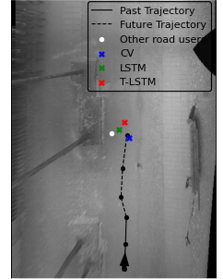
\includegraphics[width=\linewidth]{quali_results/cyc-9-1.png}
  \caption{Cyclist 9 -Frame 1}
  \label{fig:cyc9-1}
\end{subfigure}
\begin{subfigure}{0.4\textwidth}
  \centering
  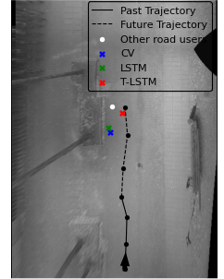
\includegraphics[width=\linewidth]{quali_results/cyc-9-2.png}
  \caption{Cyclist 9 - Frame 2}
  \label{fig:cyc9-2}
\end{subfigure}
\begin{subfigure}{0.40\textwidth}
  \centering
  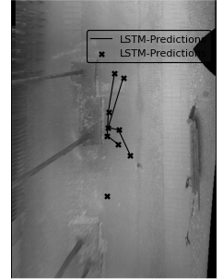
\includegraphics[width=\linewidth]{quali_results/cyc-9-l.png}
  \caption{Cyclist 9 LSTM predictions}
  \label{fig:cyc9-l}
\end{subfigure}
\begin{subfigure}{0.40\textwidth}
  \centering
  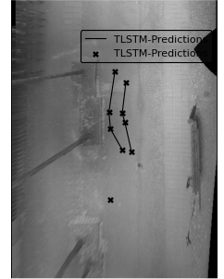
\includegraphics[width=\linewidth]{quali_results/cyc-9-t.png}
  \caption{Cyclist 9 TLSTM predictions}
  \label{fig:cyc9-t}
\end{subfigure}
\caption{Trajectories where road users don't course correct}
\label{fig:cyc9}
\end{figure}

In Figures \ref{fig:cyc9-1} and \ref{fig:cyc9-2} we clearly see that both the LSTM network and CV model predict the user to go somewhere left where there is another cyclist. On the other hand, the TLSTM network maintains some distance from the other road user on the left. Figures \ref{fig:cyc9-l} and \ref{fig:cyc9-t} refer to predictions made by both the LSTM and TLSTM network respectively. We notice that the LSTM predictions lead to some intersection in trajectories, whereas the TLSTM predictions keep the road users roughly parallel to each other. This maybe because the TLSTM network pays attention to the road user on the left and takes care to keep distance from that road user. In this dataset, head on collisions/intersections are rare as people usually move parallel to each other and in some cases maintain very less distance from each other. Therefore, we did a simulation of two pedestrians such that they are on a collision course. We compared the predictions of the LSTM and the TLSTM network to see where they are different. 


\begin{figure}[H]
\centering
\begin{subfigure}{0.4\textwidth}
  \centering
  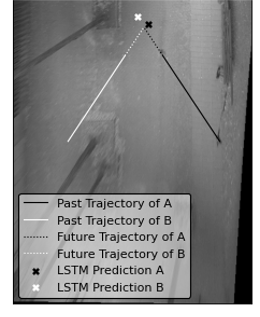
\includegraphics[width=\linewidth]{quali_results/sim-acu-l.png}
  \caption{LSTM prediction for acute collision}
  \label{fig:sim-acu-l}
\end{subfigure}
\begin{subfigure}{0.4\textwidth}
  \centering
  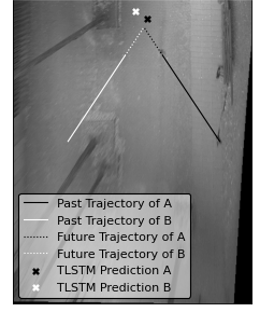
\includegraphics[width=\linewidth]{quali_results/sim-acu-t.png}
  \caption{TLSTM Prediction for acute collision}
  \label{fig:sim-acu-t}
\end{subfigure}
\begin{subfigure}{0.40\textwidth}
  \centering
  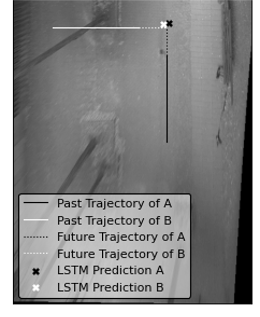
\includegraphics[width=\linewidth]{quali_results/sim-perp-l.png}
  \caption{LSTM Prediction for perpendicular collision}
  \label{fig:sim-perp-l}
\end{subfigure}
\begin{subfigure}{0.40\textwidth}
  \centering
  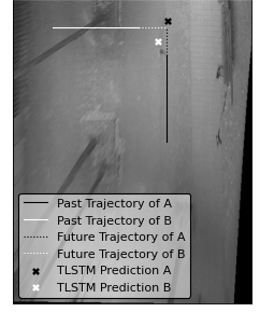
\includegraphics[width=\linewidth]{quali_results/sim-perp-t.png}
  \caption{TLSTM Prediction for perpendicular collision}
  \label{fig:sim-perp-t}
\end{subfigure}
\caption{Simulation of Trajectory Collision}
\label{fig:sims}
\end{figure}

It is noticed from Figures \ref{fig:sim-acu-l} and \ref{fig:sim-acu-t} that for an acute collision, both of them seem to course correct trajectories of $A$ and $B$. The distance between the final predictions for $A$ and $B$ is slightly greater for the TLSTM network compared to a LSTM network. However, the more interesting observation is seen in \ref{fig:sim-perp-l} and \ref{fig:sim-perp-t} where the TLSTM network avoids collision between the two road users whereas the plain vanilla LSTM predicts both road users to be approximately in the same spot. Also, given below is the attention matrix extracted from the network when it was making the prediction. It can be seen that in both these cases, road users are giving each other some attention. In the acute collision case, one of the road users gives the other road user lesser attention, even though it is expected to be symmetric for both these road users.  In the perpendicular collision case, road user A gives lesser attention to B than B gives to A. This can be reasoned on the basis that it is usually the responsibility of a person who is crossing (or moving on the lesser travelled direction) to pay attention to other road users on the main way.

\begin{table}[H]
\parbox{.45\linewidth}{
\centering
\begin{tabular}{@{}cccc@{}}
\toprule
Road User & A  & B  \\ \midrule
A  & 0.92 & 0.08 \\ 
B  & 0.63 & 0.37 \\ \midrule
%\bottomrule
\end{tabular}
\caption{Attention for the acute collision}
\label{table:attn-acute}
}
\hfill
\parbox{.5\linewidth}{
\centering
\begin{tabular}{@{}cccc@{}}
\toprule
Road User & A  & B  \\ \midrule
A  & 0.78 & 0.21 \\ 
B  & 0.58 & 0.41 \\ \midrule
%\bottomrule
\end{tabular}
\caption{Attention for perpendicular collision}
\label{table:attn-perp}
}
\end{table}









Lastly, it is interesting to look at cases where all 3 of our models fail. Figure \ref{fig:ped-entry} illustrate a pedestrian entering the building and all three models don't suggest that the pedestrian will make a sharp turn. Figure \ref{fig:ped-exit} illustrates a pedestrian leaving the building and all three models predict again that the pedestrian is going to go right and instead the pedestrian goes left. Figures \ref{fig:cyc10} and \ref{fig:cyc11} represent situations when there are abrupt turns and none of the model expect these road user maneuvers. 

\begin{figure}[H]
\centering
\begin{subfigure}{0.4\textwidth}
  \centering
  \includegraphics[width=\linewidth]{quali_results/ped-entry.png}
  \caption{Pedestrian 1 entering Frame-1}
  \label{fig:ped-entry}
\end{subfigure}
\begin{subfigure}{0.4\textwidth}
  \centering
  \includegraphics[width=\linewidth]{quali_results/ped-exit.png}
  \caption{Pedestrian 2 exiting Frame-1}
  \label{fig:ped-exit}
\end{subfigure}
\begin{subfigure}{0.40\textwidth}
  \centering
  \includegraphics[width=\linewidth]{quali_results/cyc-10.png}
  \caption{Cyclist 10 - Frame 1}
  \label{fig:cyc10}
\end{subfigure}
\begin{subfigure}{0.40\textwidth}
  \centering
  \includegraphics[width=\linewidth]{quali_results/cyc-11.png}
  \caption{Cyclist 11 - Frame 1}
  \label{fig:cyc11}
\end{subfigure}
\caption{Undetected/wrongly detected Road user maneuvers }
\label{fig:fails}
\end{figure}










\printbibliography %Prints bibliography




\end{document}
